% template adapted from https://github.com/jgm/pandoc-templates/blob/master/default.latex

%%% STYLE %%%
\documentclass[12pt,]{article}

%%% PACKAGES %%%

% fonts
\usepackage{lmodern}

% pdf
\usepackage{pdfpages}

% formulae
\usepackage{amssymb,amsmath}
\usepackage{ifxetex,ifluatex}
\usepackage{fixltx2e}
\usepackage[T1]{fontenc}
\usepackage[utf8]{inputenc}

% hyperlinks
\IfFileExists{upquote.sty}{\usepackage{upquote}}{}
\IfFileExists{microtype.sty}{%
\usepackage[]{microtype}
\UseMicrotypeSet[protrusion]{basicmath} % disable protrusion for tt fonts
}{}
\PassOptionsToPackage{hyphens}{url} % url is loaded by hyperref
\usepackage[unicode=true]{hyperref}
  \PassOptionsToPackage{usenames,dvipsnames}{color} % color is loaded by hyperref
\definecolor{maroon}{cmyk}{0, 0.87, 0.68, 0.32}
\hypersetup{
      colorlinks=true,
    linkcolor=maroon,
    citecolor=blue,
    urlcolor=blue,
      breaklinks=true}
\urlstyle{same} % don't use monospace font for urls

% geometry
\usepackage[left=3cm,right=2cm,top=2cm,bottom=2cm]{geometry}
\renewcommand{\baselinestretch}{1.1}

% Bibliography
\usepackage{natbib}
\bibliographystyle{plainnat}

% Tables
\usepackage{longtable,booktabs}
% Fix footnotes in tables (requires footnote package)
\IfFileExists{footnote.sty}{\usepackage{footnote}\makesavenoteenv{long table}}{}

% graphics
\usepackage{graphicx,grffile}
\makeatletter
\def\maxwidth{\ifdim\Gin@nat@width>\linewidth\linewidth\else\Gin@nat@width\fi}
\def\maxheight{\ifdim\Gin@nat@height>\textheight\textheight\else\Gin@nat@height\fi}
\makeatother
\setkeys{Gin}{width=\maxwidth,height=\maxheight,keepaspectratio}

% indent
\IfFileExists{parskip.sty}{%
\usepackage{parskip}
}{% else
\setlength{\parindent}{0pt}
\setlength{\parskip}{6pt plus 2pt minus 1pt}
}

% prevent overfull lines
\setlength{\emergencystretch}{3em}  
\providecommand{\tightlist}{%
\setlength{\itemsep}{0pt}\setlength{\parskip}{0pt}}

\setcounter{secnumdepth}{0}

% paragraphs
\usepackage{titlesec}
\let\oldsection\section
\renewcommand\section{\newpage\oldsection}
\titleformat{\section}
{\huge\center\scshape}{\thesection}{1em}{}[{\titlerule[0.8pt]}]
\titleformat*{\subsection}{\LARGE\bfseries}
\titleformat*{\subsubsection}{\Large\bfseries}
\titleformat*{\paragraph}{\large\bfseries\itshape}
\titleformat*{\subparagraph}{\normalsize\itshape}

% citations
\usepackage{epigraph}

% set default figure placement to htbp
\makeatletter 
\def\fps@figure{htbp}
\makeatother

%%% BODY %%%
\usepackage{amsthm}
\newtheorem{theorem}{Theorem}[section]
\newtheorem{lemma}{Lemma}[section]
\theoremstyle{definition}
\newtheorem{definition}{Definition}[section]
\newtheorem{corollary}{Corollary}[section]
\newtheorem{proposition}{Proposition}[section]
\theoremstyle{definition}
\newtheorem{example}{Example}[section]
\theoremstyle{definition}
\newtheorem{exercise}{Exercise}[section]
\theoremstyle{remark}
\newtheorem*{remark}{Remark}
\newtheorem*{solution}{Solution}
\begin{document}

% First pages
  % First page
  
\includegraphics{images/logos}
  
  \begin{center}
  \Large{\textbf{Université des Antilles}} \\
    \vspace*{\stretch{1}}
    \LARGE{\textbf{Mémoire de stage}} \\
    \vspace*{\fill}
    \large{présenté par} \\
    \large{Nino PAGE} \\
    \vspace*{\fill}
    \large{pour obtenir le diplôme national de master} \\
    \large{parcours Ecologie des écosystèmes Tropicaux naturels et exploités (ECOTROP)} \\
    \small{spécialité : Ecologie des Forêts Tropicales} \\
    \vspace*{\fill}
    \large{Sujet :} \\
    \Large{\textbf{Modeling the impacts of selective logging on tropical forests: A first attempt with TROLL, in French Guiana}} \\
    \vspace*{\fill}
    \large{soutenu publiquement le 25 Juin 2017} \\
    \large{à Kourou} \\
    \vspace*{\fill}
    \large{Encadré par :} \\
    \vspace*{\fill}
    Dr Stéphane TRAISSAC  \emph{Tuteur de stage} \\
    Dr Bruno Hérault  \emph{Co-encadrant} \\
    Dr Sylvain Schmitt  \emph{Co-encadrant} \\
    Dr Maguy DULORMNE  \emph{Enseignant-référent} \\
    \vspace*{\stretch{1}}
  \end{center}
  
  % Second page
  \newpage
  \vspace*{\fill}
  \epigraph{L\textquoteright arbre est un organisme tellement généreux qu’il offre son ombre à ceux qui viennent l\textquoteright abattre.}{\textit{Francis Hallé}}
  \vspace*{\fill}
  \emph{Les opinions émises par les auteurs sont personnelles et n'engagent ni EcoFoG, ni le CNRS.}\\
  \emph{Une version web de ce document sera diponible à l'adresse suivante : \url{https://riodinino.github.io/master-thesis/}.}
  \newpage

\tableofcontents

\section*{Résumé}\label{resume}
\addcontentsline{toc}{section}{Résumé}

Les forêts tropicales abritent la moitié de la biodiversité terrestre
mondiale, fournissent d'importants services écosystémiques à l'humanité,
et sont un important réservoir de carbone. Ces forêts font face à de
nombreuses menaces, dont la déforestation à des fins agricoles, et
l'exploitation forestière séléctive. Cette dernière a affecté ou
affectera la majorité des forêts tropicales, et a longtemps été une
pratique incontrôlée \citep{Nasi2009}. La Gestion Forestière Durable a
été mise en avant pour tenter de résoudre ce problème, s'appuyant
notamment sur les principes de l'Exploitation à Faible Impact
\citep[EFI,][]{Putz2008} et des incitations financières, comme le
programme REDD+. Cependant, certains auteurs ont remis en question la
durabilité réelle d'une telle exploitation
\citep{Kormos2012, Pearce2003}. Evaluer l'impact des pratiques
forestières est une tâche difficile, au vu des échelles de temps
impliquées. En complément des efforts de suivi, la modélisation peut
s'avérer utile pour fournir un aperçu des effets de l'exploitation
forestière à plus long terme.\\
TROLL est un modèle spatialement explicite, individu-centré, qui simule
un grand nombre d'espèces d'arbres. TROLL offre d'intéressantes
perspectives en écologie théorique et appliquée
\citep[\citet{Chave1999b}]{Marechaux2017a}. Nous avons exploré le
potentiel de ce modèle pour simuler l'exploitation sélective, et
explorer la durabilité de plusieurs scénarios. Nous avons commencé par
paramétrer 547 espèces à partir de la base de données BRIDGE
\citep{Baraloto2010}, pour simuler d'importantes étendues de forêt, et
avons ensuite essayé de réaliser une évaluation et calibration des
trajectoires post-coupe simulées, en partaint de données réelles. La
calibration fut impossible à cause d'une mortalité éxagérée dans les
forêts d'entrées, pendant les premières années de simulation. Nos
analyses suggèrent que TROLL a une structure spatiale différente de
celle de vraies forêts, peut être à cause d'une sur-estimation de la
compétition pour la lumière, le rendant inadapté à simuler à partir de
vraies données pour le moment. Nous avons adapté la version existante du
module simulant l'exploitation dans TROLL, pour implémenter plusieurs
pratiques et paramètres sylvicoles. Nous avons réalisé un premier jeu de
simulations sur deux forêts ayant des volumes de départ contrastés,
durant 5 rotations. Nos résultats indiquent que l'exploitation
sélective, telle qu'elle est pratiquée en Guyane Française, pourrait
mener à un épuisement des volumes totaux d'espèces commerciales, ainsi
qu'a une baisse du stock de carbone au fil des récoltes, et cela même
pour des rotations de 65 ans, avec des intensités de 20\(m^3\) et les
techniques de l'EFI. Ces résultats sont cependant préliminaires et
manquent de réplication, ils doivent donc être interprétés avec
précaution. Des analyses plus poussées sur des scénarios plus nombreux
sont requises afin de confirmer et affiner nos résultats. TROLL, combiné
avec le modèle d'exploitation que nous avons mis à jour, présente un
potentiel promettent pour explorer différents scénarios sylvicoles, et
répondre à des problématiques appliquées.

\section{Abstract}\label{abstract}

Tropical forests shelter half the terrestrial biodiversity worldwide,
provide important services to humanity and are a major reservoir of
carbon. These forests face numerous threats, among others deforestation
for agriculture and selective logging. Selective logging affected or
will affect the majority of tropical forest outside protected areas, and
has long been an uncontroled predatory practice \citep{Nasi2009}.
Sustainable Forest Management (SFM) has been promoted to answer this
issue, relying on Reduced Impact Logging \citep[RIL,][]{Putz2008}, and
financial incentives such ad REDD+. However, some authors asked whether
these techniques are sustainable \citep{Kormos2012, Pearce2003}.
Assessing the sustainability of Forest Management difficult task,
because of the efforts needed by field studies, and time scales
involved. To complement monitoring efforts, the use of models can
provide valuable insights of longer-term effects of selective logging.
TROLL is an individual-tree-based, spatially explicit forest model that
uses functional traits to simulate the life cycle of a wide range of
tree species. TROLL offers promising perspectives in studying ecological
theories and applied problems
\citep[\citet{Chave1999b}]{Marechaux2017a}. We explored the potential of
this model to simulate selective logging and assess the sustainability
of different scenarios. We preliminarily parametrized 547 species from
the BRIDGE dataset \citep{Baraloto2010} to simulate large forest plots,
and we attempted to evaluate and calibrate the simulated post-logging
trajectories inputting real forest censuses in the model. The
calibration was impossible because of exagerated mortality in the
inputted forests during the first years of simulation. Spatial structure
analysis suggest that TROLL has a different spatial structure than real
forests, maybe due to overestimation of competition for light, thus
making unadapted the use of real data inputs for now. We adapted the
existing version of the module that simulates selective logging in
TROLL, to implement cutting cycles, conventional logging, and
designation based on timber interest ranks. We did a preliminary set of
simulations on two forests that had contrasted timber volumes, to assess
the importance of silviculture parameters over five cutting cycles. Our
results indicate that selective logging, as applied in French Guiana and
neighboring countries, may lead to a depletion of total timber stocks
and high-grade species, along with a decrease of carbon stocks over
harvests, even for 65 years cutting cycles with 20\(m^3\) harvested and
RIL techniques. However, our results are preliminary, lack replication,
and thus have to be interpreted carefully. Further, extensive analyses
are needed to confirm and refine our findings. TROLL, combined with the
logging model we updated, has a promising potential to explore a wide
range of silviculture scenarios, and adress applied problematics.

\section{Introduction}\label{introduction}

Tropical forests shelter over half the terrestrial species present on
Earth and provide numerous goods and services, many of which have
essential economic or societal value \citep{Foley2007, Myers1997}. They
represent a major carbon reservoir, holding up to half the estimated 558
Pg stored in vegetation worldwide \citep{Houghton2005}. Tropical forests
are currently facing multiple perils, including deforestation for
pasture or food crops, and forest degradation, for example, selective
logging or fires \citep{Houghton2012}. Recently, \citet{Pearson2017}
estimated a yearly total of 8.29 \(Pg\) carbon loss from deforestation
and forest degradation worldwide. Although deforestation is easy to
evaluate with satellite images, and have raised much concern over past
decades, estimating and regulating the extent and emissions from forest
degradation is critical, yet challenging\citep{Herold2011}. Selective
logging is the targetted harvest of a reduced number of individuals,
belonging to high value timber species. Selective logging is an
important cause of forest disturbance. It affected or will affect the
majority of tropical forest outside protected areas \citep{Putz2012}. In
2011, 403.000.000 hectares were officially designated for timber
extraction in tropical rainforests \citep{Blaser2011}. Two years
earlier, \citet{Asner2009} reported that the annual rates (regarding the
area) at which these forests are selectively logged approaches 20 times
those of deforestation. It is especially the case in the Amazon Basin,
that encompasses half of all remaining tropical moist forest, and is an
important carbon reservoir estimated to hold \emph{ca.}90 PG of
above-ground carbon \citep{FAO2010, Saatchi2007, Malhi2006}. Amazonia
has been severely deforested since the early 1970s, and although overall
rates substantially reduced \citep[ \emph{in}
\citet{Rappaport2018}]{INPE2015}, a recent rise of small-scale
deforestation, close to forest degradation, was recently noticed
\citep{Kalamandeen2018}. In the Brazilian Amazon, selective logging
impacted \emph{ca.} 2 \(Mha.y^{−1}\) between 1999 and 2002
\citep{Asner2005}, raising resulting in emissions of about 90
\(TgC.y^{−1}\), \emph{i.e.} 15-19\% higher than reported from
deforestation alone over the same period \citep{Huang2010}.

Selective logging has long rimed with irresponsible cutting
\citep{Kormos2012}, and poorly regulated harvesting. Governmental and
global policies, more than two decades ago, engaged in a collective
endeavor to limit this trend with the introduction of Sustainable Forest
Management {[}SFM; United Nations, 1992{]}. Later on, projects such as
REDD+ \citep[Reducing Emissions from Deforestation and forest
Degradation,][]{UNFCCC2008} linked SFM and climate change to pursue one
common cause, using financial incentives. In parallel, aset of
techniques and planning guidelines were introduced to mitigate the
adverse effects of conventional selective logging, under the name
``Reduced impact logging'' (RIL). RIL is increasingly implemented and
promoted as a cornerstone to achieving both ecologically and
economically viable forest management \citep{Putz2008}. It is somehow
seen as a reasonable compromise between clearcutting and outright
protection \citep{Putz2012}. Some authors argue in favor of RIL's
potential to sustain essential ecosystemic and services, such as the
ecosystem's conservation value, above-ground biomass, and timber yields
\citep{Putz2012}. Conversely, Others insist on the apparent
non-sustainability of current practices, and affirm that they are only
leading to depletion of timber volumes, carbon stocks, and biological
diversity, due to mismatches between minimum economic viability, and
subtle ecosystem functioning - on timescales far beyond ours
\citep[see][ and \citet{Kormos2012}]{Nasi2009}.

There is no available dataset for more than two cutting cycles. We have
insights that resource use-up is ensured at the second or third cutting
cycle \citetext{\citealp{Kormos2012}; \citealp[but see][]{Putz2012}}.
Data on forest biomass recovery has also intensively been studied,
yielding contrasted conclusions worldwide. Likely, carbon stock is the
first global ecosystemic variable to be recovered after a disturbance
{[}Sist et al., 2015{]}, but the nature of the stands is very different.
A majority of commercial timber species (and mature forest trees) are
long-lived, shade-tolerant species, rely on complex pollination and
dispersal strategies to maintain viable population sizes, and occur low
concentration of individuals per spatial unit. They are, in many cases,
outcompeted by pioneers, light-responsive species, which contribute
carbon stocks transiently and may slow others regeneration
\citep{Nasi2009}.

These observations are for short time-scales. To produce at least
conservative estimates of what our actions yield, over time-scales that
we cannot apprehend, the use of models is a relevant approach. After
all, this is the only source of \emph{a priori} information that we can
use to orientate long-term management decisions. Most simulation studies
on selective logging focused on carbon
\citep{Piponiot2016, Rutishauser2015, Huang2008} with more or less
large-scale approaches. Up to now, relatively few simulation studies
addressed the sustainability of selective logging at the plots' scale,
especially for long timescales. \citet{Sist2007} and \citet{Dauber2005}
simulated growth and mortality of remaining stands on logged plots, in
the Eastern and Western Amazon, respectively. In the Paragominas
(Brasil), \citet{Valle2007} used individual-based models to assess
timber yields over cutting cycles, but used only 10 species groups,
which is somehow restrictive \citep[see][]{Marechaux2017}
\citet{Huth2001}, did a relatively complete assessment of cutting cycle
durations and target volumes on Malaysian dipterocarp forests, further
discussed in \citet{Huth2003}, but again using only 10 species groups to
model hyper-diverse forests. \citet{Gourlet-Fleury2005a} also used an
individual-based model to simulate timber stocks recovery for
\emph{Dicorynia guianensis}, the principal harvested species in French
Guiana \citep{Guitet2011}. There is a need for models either enabling
simulation of selective logging for large time scales (over centuries)
and integrating fine-scale processes and species diversity.
Individual-based and spatial-explicit models are thus offering a
perspective to address this need.

TROLL is an individual-based forest simulator that jointly simulates
species diversity and carbon dynamics \citep{Marechaux2017a}, over time
scales ranging from years to centuries. It explicitly accounts for the
influence of species-specific functional traits and competition for
light on individuals life cycle (growth, mortality, recruitment,
reproduction). We used TROLL to bring a first contribution to the
assessment of selective logging sustainability in French Guiana.

Our aims were: * to get as close as possible to the actual logged
forests in terms of diversity; * to model selective logging
realistically, given field reality and the model limits; * to
preliminary explore of possible scenarios for the wood industry in
French Guiana; * to make a generic tool that allows testing more
scenarios.

To match these goals, we followed four steps. We first inferred a new
species input dataset to simulate more species in French Guianese
forests. We then attempted a validation and calibration of post-logging
recovery with TROLL, using real censuses from logged and undisturbed
plots of the Paracou disturbance experiment. Subsequently, we updated
the existing selective logging module to include features such as
multiple cutting cycles, conventional logging, designation with species
interest ranking, and continuous monitoring of merchantable trees.
Finally, we did a pilot-experiment, simulating two cutting cycles, two
target volumes, three diversification scenarios, RIL and CL, on two
primary forests with contrasted initial timber stocks.

\section{TROLL model}\label{troll-model}

\subsection{Overview}\label{overview}

TROLL simulates every tree starting from 1 meter high (formerly, 1 cm
dbh) in a spatialized light environment, where every process of the
trees life cycle are modeled according to global rates, species-specific
traits, and photosynthetic rates influenced by individual-level light
incomes. TROLL can thus be defined as an individual-based and spatially
explicit forest growth model, along with SORTIE
\citep{Pacala1996, Uriarte2009} and FORMIND \citep{Fischer2016}.
Actually, TROLL can be qualified with many adjectives. The most
important among them are individual tree-based, spatially-explicit, and
process- and physiology-based.

TROLL simulates two classes of objects: species, and trees. Trees are
simulated in a tridimensional (voxel) space of one-meter resolution, in
which the light environment is explicitly computed. One tree can settle
in each horizontal pixel of 1\(m^2\). Each tree has a number of
attributes, which we can classify into two categories: biometric, state
variables, and species-specific variables (see Figure
\ref{fig:TROLLtree}.

\begin{figure}
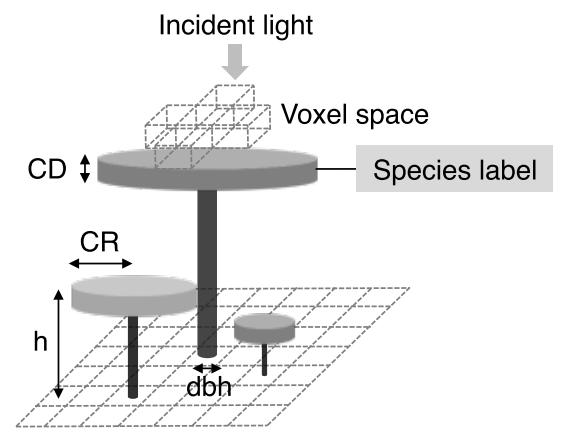
\includegraphics[width=0.6\textwidth]{images/TROLLtree} \caption{Individuals tree inside TROLL explicit spatial grid from @Marechaux2017a. Tree geometry (crown radius CR, crown depth CD, height h, diameter at breast height dbh) is updated at each timestep (1 months) using allometric relationship with assimilated carbon allocated to growth. Each tree inherits a species label linking to its species-specific attributes. Light is computed explicitly at each timestep for each voxel, and trees are asymetrically shading each-other.}\label{fig:TROLLtree}
\end{figure}

The firsts encompass tree age, diameter at brease height (\(dbh\)),
height (\(h\)), crown radius (\(CR\)) and depth (\(CD\)), leaf area
(\(LA\)). The second encompass five functional traits and two allometric
parameters (\emph{cf.} Table \ref{tab:traits}). Species are linked to
trees with by a species label, which is inherited from the parent
(mother) tree.

\begin{longtable}[]{@{}lll@{}}
\caption{\label{tab:traits}Species-specific parameters used in TROLL from
\citet{Marechaux2017a}. Data originates from the BRIDGE
\citep{Baraloto2010} and TRY \citep{Kattge2011}
datasets.}\tabularnewline
\toprule
Abbreviation & Description & Units\tabularnewline
\midrule
\endfirsthead
\toprule
Abbreviation & Description & Units\tabularnewline
\midrule
\endhead
\(LMA\) & leaf mass per area & \(g.m^{-2}\)\tabularnewline
\(N_m\) & leaf nitrogen content per dry mass &
\(mg.g^{-1}\)\tabularnewline
\(P_m\) & leaf phosphorous content per dry mass &
\(mg.g^{-1}\)\tabularnewline
\(wsg\) & wood specific gravity & \(g.cm^{-3}\)\tabularnewline
\(dbh_{thresh}\) & diameter at breasth height threshold &
\(m\)\tabularnewline
\(h_{lim}\) & asymptotic height & \(m\)\tabularnewline
\(a_h\) & parameter of the tree-height-dbh allometry &
\(\mu\)\tabularnewline
\bottomrule
\end{longtable}

Tree geometry is derived from its diameter according to allometric
relations, whereas leaf area varies dynamically within each tree crown.
Contrasting with other forest simulators, TROLL models tree growth as
the result of an explicitly computed carbon balance between assimilation
by photosynthesis, emissions from respiration, and allocation to the
different tree compartments. Assimilation is computed according to
climate input data, over half-hourly periods of a representative day,
and influences the simulated environment at the next time step, which
defaults to one month. Seeds and seedlings are not explicitly modeled
and are considered part of a seedling/seed pool. Every tree belongs to a
species through a species label, and thus shares common species features
that are inherited from the mother tree through the seed. The species
label established the correspondence between a tree and species-specific
parameters, i.e.~trait values obtained from field measurements (and
inference). Currently, soil processes and topography are not explicitly
modeled. Their overall influence on a real forest at a plot's scale is
implicit, partly accounted for when using site-specific species
datasets.

\section{Including more species in TROLL
simulations}\label{including-more-species-in-troll-simulations}

\subsection{Introduction}\label{introduction-1}

Biodiversity affects most of the ecosystemic characteristics, among
others productivity, stability, resistance to invasion
\citep{Lyons2001, Huston2001}. Recent advances in Functional Ecology
suggest that the most relevant approach to study ecosystem functioning
is through its functional composition, that can be assessed using
functional traits. Functional traits are formally defined as
morpho-physio-phenological traits that indirectly impact fitness via
their effect on growth, survival, and reproduction \citep{Violle2007}.
Accounting for functional traits and their effects on processes is
necessary to model forest dynamics with a finer accuracy. Classical
models often use a limited number of species groups defined according to
restrictive criteria \citep{Marechaux2017a}. TROLL directly uses 5
functional traits (LMA, Nmass, Pmass, and wsg) and 2 allometric
parameters at the species-specific level. All are obtained from real
data.

We included more species to the existing dataset used for TROLL
simulations. This choice was motivated by both theoretical and practical
reasons. The aims were either to enhance the coverage (in number of
trees) for Paracou simulations (see next section) and to have enough
species to simulate large plots, for the logging experiment. We
hierarchically inferred species-specific means for leaf traits, stem
traits and allometric parameters, with the BRIDGE dataset. We estimated
the 99th quantiles of species diameter from the whole Guyafor dataset,
pooled with BRIDGE. We used Predictive Mean Matching to complete the
dataset beforehand, due to a variable -Pmass- that considerably limited
our possibilities. The model blueprints were generously provided by
Fabian Fischer (EDB, Toulouse).

\subsection{Context and Problem}\label{context-and-problem}

\subsubsection{The initial species list}\label{the-initial-species-list}

TROLL's current species-specific trait dataset contains 8 variables:
\(LMA\), \(Nmass\), \(Pmass\), \(wsg\), \(hmax\), \(dmax\), \(ah\), and
\(Freg\) (see table \ref{tab:traits}, in the previous section). We
decided to let apart the regional frequency of a species, which are
adapted for each simulation depending on the forest composition and
simulation aims.

\subsection{Can we represent Paracou plots composition with TROLL's
species list
?}\label{can-we-represent-paracou-plots-composition-with-trolls-species-list}

Paracou plots display a high proportion of species that are absent of
TROLL dataset (Figure \ref{fig:paracousummary}). Based on preliminary
exploration of the Paracou dataset, we noticed that the proportion of
individuals belonging to missing species is slightly reducing over time,
possibly linked with an increase in botanical determination reliability.
This proportion is rather low compared to the proportions of missing
species. However, such proportions were questioning the \emph{a priori}
validity of our intent to simulate real forest plots. These species are
mainly less common ones and may be absent either because they were not
present in the plots sampled in BRIDGE or because their number of
observations did not allow including them.

\begin{figure}
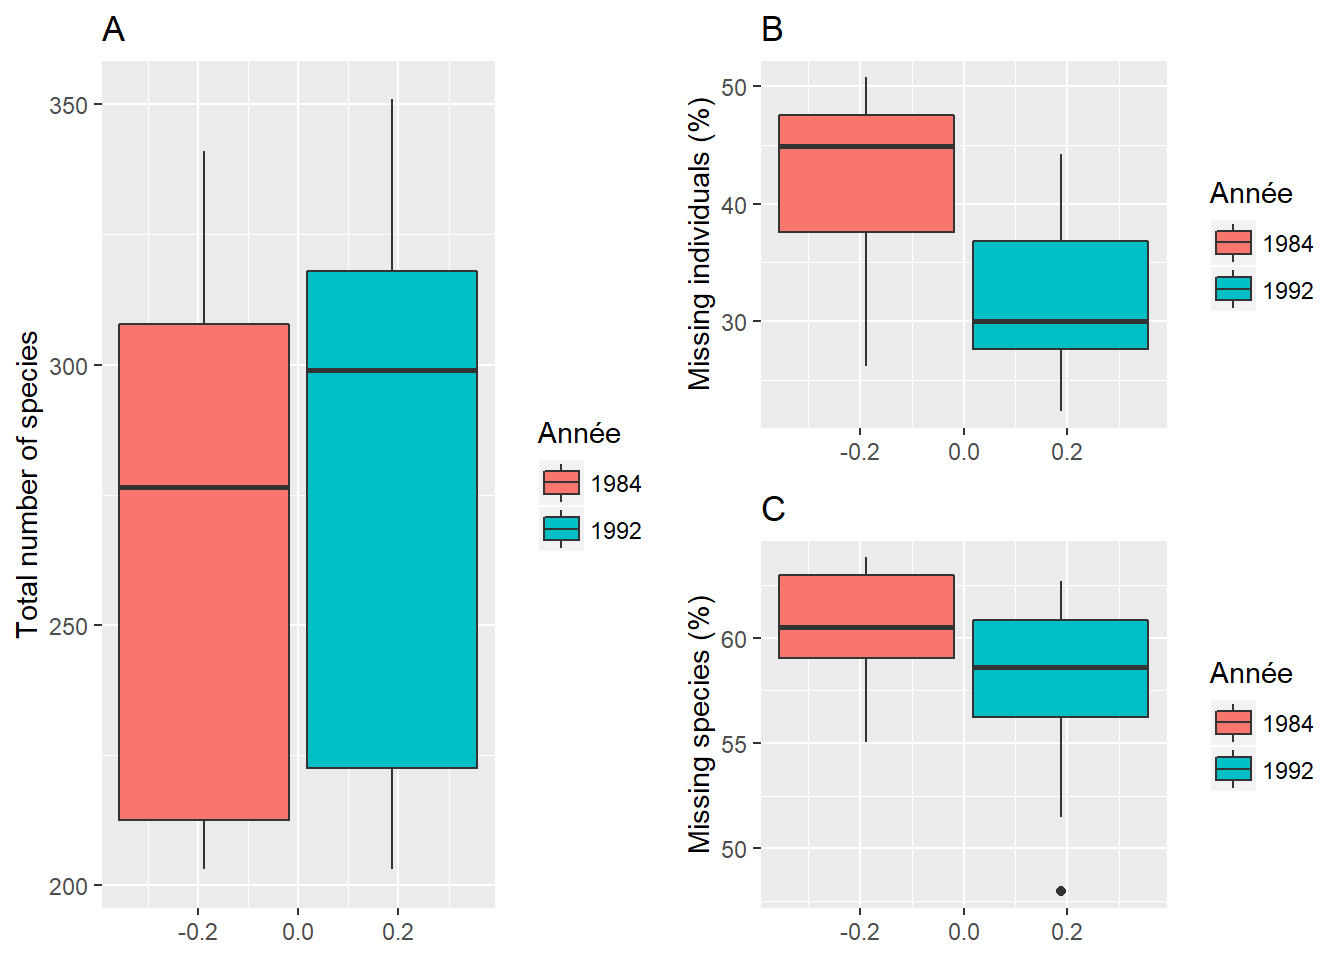
\includegraphics[width=0.6\textwidth]{master-thesis_files/figure-latex/paracousummary-1} \caption{ Total number of species, proportions of missing species and individuals in two censuses (1984,1992) for twelve Paracou Plots (1-12). A: Total number of species in the plots, at the plot scale; B: Proportion of individuals belonging to missing species; C: Proportion of missing species; All are computed at the plot scale. Colors represent the census years (red: 1984, blue: 1992)}\label{fig:paracousummary}
\end{figure}

\paragraph{Missing species and
individuals}\label{missing-species-and-individuals}

\paragraph{Functional
representativity}\label{functional-representativity}

Figure \ref{fig:representat} compares the distribution of LMA and wsg
for BRIDGE and species from TROLL's list that occur in Paracou. These
traits are linked to construction costs for the trees and are part of
the leaf and wood economics spectra \citep{Wright2004, Chave2009}.
According to \citet{Baraloto2010}, both spectra are decoupled and
represent two components of the plants' strategy. In TROLL, LMA is
linked to leaf lifespan, photosynthesis In Figure \ref{fig:representat},
the fraction of TROLL species list that matches with Paracou (137
species) is rather representative of the bridge dataset (which we assume
to be itself well representative of the real forests' functional traits
ranges). However, each plot had from 70 to 115 species matching with
those of TROLL, out of 300 species present As explained above, not only
the number of species matching those of TROLL was low, but also, the
corresponding number of individuals was problematic. We thus decided to
perform a new trait means inference to reach a better representativity,
and to simulate Paracou plots.

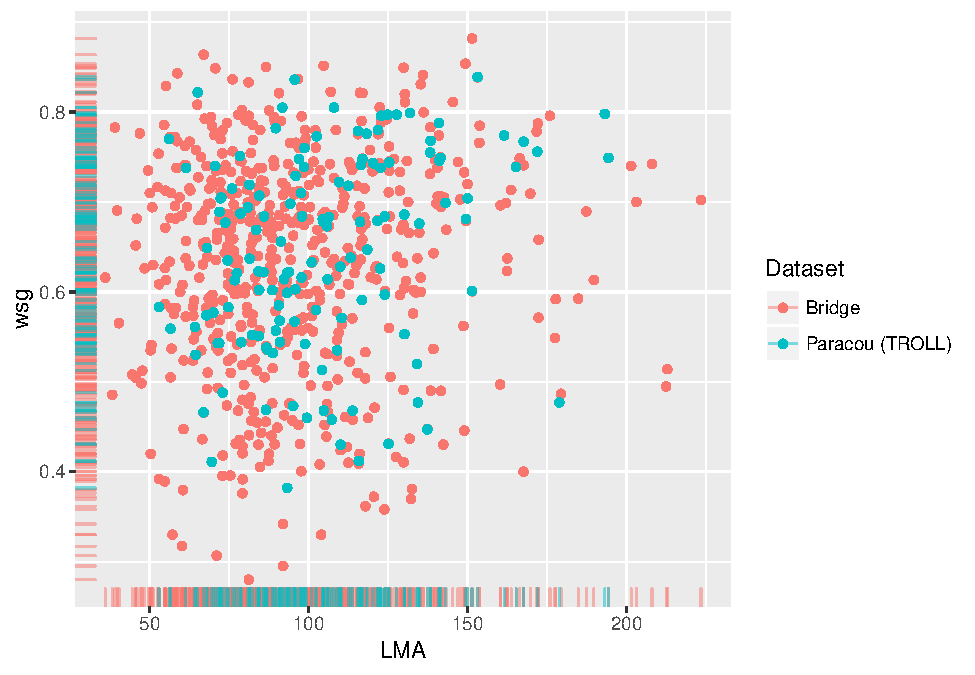
\includegraphics[width=0.6\textwidth]{master-thesis_files/figure-latex/representat-1}

\subsection{How to parametrise more species
?}\label{how-to-parametrise-more-species}

\subsubsection{Datasets}\label{datasets}

We used the BRIDGE trait database \citep{Baraloto2010, Baraloto2012}
which was further completed by \citet{Marechaux2017}, to infer leaf,
stem and allometric parameters. We used both BRIDGE and Guyafor datasets
to estimate dmax, as the 99th percentil of speces diameters. The BRIDGE
dataset contains measurements for ten leaf and stem traits, with a total
of 4709 individuals. One of the strengths of BRIDGE is that nine plots
were sampled exhaustively, thus providing an exceptional representation
of the French Guianese forests functional composition for
\textgreater{}10cm dbh trees. However, another feature of the BRIDGE
dataset is that the plots sampled are tropical rainforest: the dataset
contains numerous species with a majority of rare (\textgreater{}4
observations) and a minority of highly dominant (\textgreater{} 200
observations) species. We used six individual-level traits and
characteristics, namely: LMA, Nmass, Pmass, wsg, H, d
(\ref(tab:traits)).

\begin{longtable}[]{@{}lllll@{}}
\caption{\label{tab:tablebridge2}Summary table of the trait data obtained
from the BRIDGE database. The two last rows ``Total'' and ``LMA, N,
wsg'' are the complete observation for all traits and with P excluded,
respectively.}\tabularnewline
\toprule
Trait & Unit & N (complete) & Missing data & Species\tabularnewline
\midrule
\endfirsthead
\toprule
Trait & Unit & N (complete) & Missing data & Species\tabularnewline
\midrule
\endhead
LMA & g.cm\^{}\{2\} & 4460 & 265 & 642\tabularnewline
Nmass & mg.g\^{}\{-1\} & 2928 & 1797 & 537\tabularnewline
Pmass & mg.g\^{}\{-1\} & 931 & 3794 & 270\tabularnewline
wsg & g.cm\^{}\{-3\} & 2875 & 1850 & 630\tabularnewline
Height & m & 4399 & 326 & 645\tabularnewline
dbh & m & 4597 & 128 & 663\tabularnewline
Total & - & 651 & - & 251\tabularnewline
LMA, N, wsg & - & 1726 & - & 505\tabularnewline
\bottomrule
\end{longtable}

The dataset we used contains significant amounts of missing data, as the
majority of functional trait databases \citep{Taugourdeau2014}. Still,
we can infer a high number of species means for LMA, Nmass, wsg and
height-diameter allometries. For Pmass, however, very few observations
are available compared to other variables. It is by far the most
limiting variable. Indeed, out of the 270 species, the overwhelming
majority of them are singletons (see Figure \ref{fig:phosphorus} in the
second Appendix section). \citet{Marechaux2017a} have further completed
this dataset, probably with TRY database \citep{Kattge2011} to achieve
parametrization for 163 species in TROLL.

\subsubsection{Preliminary completion with Predictive mean
matching}\label{preliminary-completion-with-predictive-mean-matching}

We used aPredictive Mean Matching algorithm (described in the third
Appendix), implemented in the R-package mice \citep{Buuren2011}. We used
the default \(k=5\) (the number of matched cases per iteration) proposed
in the mice package and repeated the imputations ten times, then pooled
the datasets and averaged the obtained proposals for missing values. To
improve predictive power based on inter-trait correlation, we included
additional variables that were correlated with our target variables, and
selected with an automatic, stepwise linear model comparison procedure:
leaf toughness, leaf thickness, SPAD (a proxy of chlorophyll content),
and leaf carbon content. Palms were excluded from the analysis
beforehand since there are not currently modeled with TROLL. Individuals
belonging to indeterminate genera and species were discarded (except
those present in Paracou, for example, \emph{Symphonia sp.1}), as well
as individuals with only one trait measured or high taxonomic
uncertainty. Moreover, we clustered the observations according to
taxonomical levels: Imputations were performed at the genus level if
more than 30 complete observations were available. If not, imputation
was made at the family level, with the same threshold. Monogeneric and
underrepresented families were treated at the overall level. This
separation aimed at reducing the errors due to using overall
relationships to infer values.

We obtained a completed dataset of 4245 observations, with a total of
599 represented species, which is less than the original species number
for LMA and wsg. Pmass have more inferred values than actual measures in
this completed dataset.

\subsubsection{Hierarchical modeling
framework}\label{hierarchical-modeling-framework}

We used a simple but efficient modeling framework, which was blueprinted
by Fabian Fisher (\emph{pers. comm.}), to hierarchically infer species
means and take advantage of every available observation.

The idea is quite simple: for a trait (or an allometric parameter), the
value observed in individuals depends on a species mean (modulo a
variance, assumed homogenous across species), which is itself related to
an higher-level grouping entity mean. For example, we can consider that
species mean depends on genus mean, that is itself related to the family
mean, and so on up to the overall observed mean (\emph{i.e.} regardless
to grouping entities). The most critical choices here are the number of
grouping entities, an appropriate distribution, and informative priors
for the target parameters.

After testing several configurations, we decided to stick with only two
layers, namely species and overall levels. The main reason for this
choice was parsimony. Genera means, variance, and species raw/actual
deviation from its genus mean represented a high number of extra
parameters, which is excessive compared to the predictive power
enhancement it represents. This was confirmed by a quick comparison
using the WAIC criterion, that confirmed our intuition (data not shown)

\subsubsection{Leaf and stem traits}\label{leaf-and-stem-traits}

To infer species mean traits, we used two types of hierarchical models.
Both accounted for two layers only, for reasons of parsimony: adding
grouping variables (Genus or Family) did not bring significant
improvement considering the number of parameters added.

We used the following model:

\begin{equation}
  X_{sp} \sim \mathcal{N}(\mu_{sp}, \sigma_{intra})
  \label{eq:leaftraits1}
\end{equation}

Where, for individuals belonging to species \(s\), and a given trait (or
log-transformed trait) \(X\), the \(X\) attribute of these individual
follows a \(Gaussian\) prodability distribution, of parameters
\(\mu_{sp}\), a species-level trait mean, and \(sigma_{intra}\), the
intraspecific variance (here assumer to be homogen among species).
Moreover:

\begin{equation}
  \mu_{sp} \sim \mathcal{N}(\mu_{tot}, \sigma)
  \label{eq:leaftraits2}
\end{equation}

The species mean \(\mu_{sp}\) itself is normally distributed, depending
on an overall mean \(\mu_{tot}\) and an overall variance \(\sigma\).

\subsubsection{Michaelis-Menten hierarchical
model}\label{michaelis-menten-hierarchical-model}

In TROLL model, the allometries used to model trees height/dbh
relationship is a Michaelis-Menten form, defined as:

\begin{equation}
  \hat h = log(\frac{h_{max_{sp[i]}}*dbh[i]}{dbh[i]+a_h}
  \label{eq:michaelis}
\end{equation}

Originally, the model provided by Fabian has the form:

\begin{equation}
  [log(h_i) |sp_i; dbh_i] \sim \mathcal{N}([\hat h_i | sp_i; dbh_i], \sigma)
  \label{eq:michaelis2}
\end{equation}

Where \(h\) is the observed height for tree \(i\), which varies
lognormally around \(\hat h_i\), the expectation of its height knowing
its species \(sp_i\) and diameter \(dbh_i\), with variance \(\sigma\).
\(\hat h_i\) is computed with:

\begin{equation}
  [\hat h_i | sp_i; dbh_i] = log(\frac{1}{(\frac{1}{h_{max_{sp_i}}}+\frac{1}{\beta_{sp_i}*dbh_i})})
  \label{eq:leaftraits1}
\end{equation}

Where \(h_{max_{sp_i}}\) is the asymptotic height of species \(i\), and
\(\beta_{sp_i}\), a shape parameter of the model. Both are define by:

\begin{equation}
  \beta_{sp[i]}  \sim \mathcal{N}(\bar \beta, \sigma_{\beta}) and  h_{max_{sp[i]}}  \sim \mathcal{N}(\bar h_{max}, \sigma_{\beta}) 
  \label{eq:michaelis2}
\end{equation}

Equation \eqref{eq:leaftraits2} can be rewritten to the classical
Michaelis-Menten form:

\begin{equation}
  \hat h = log(\frac{h_{max_{sp[i]}}*dbh[i]}{dbh[i]+\frac{h_{max_{sp[i]}}}{\beta_{sp[i]}}}
  \label{eq:leaftraits2}
\end{equation}

Thus, with \(\frac{h_{max_{sp[i]}}}{\beta_{sp}}\) corresponding to
\(a_h\) in the equation \eqref{eq:michaelis}

\subsection{More species for TROLL}\label{more-species-for-troll}

We obtained a new set of 599 species means for Nmass, Pmass, wsg and LMA
using the inference procedure. Allometric parameters and \(dmax\)
limited the final dataset for TROLL to 547 species. 347 of those species
matched with Paracou species. Figure \ref{fig:representatfin} shows that
the new species set has a better coverage of wsg and LMA distributions.
The histograms for each trait are available in the second Appendix
sections. Overall, the inferred species set allowed to better represent
trait distributions in TROLL, and enhanced the coverage for Paracou.

\begin{figure}
\centering
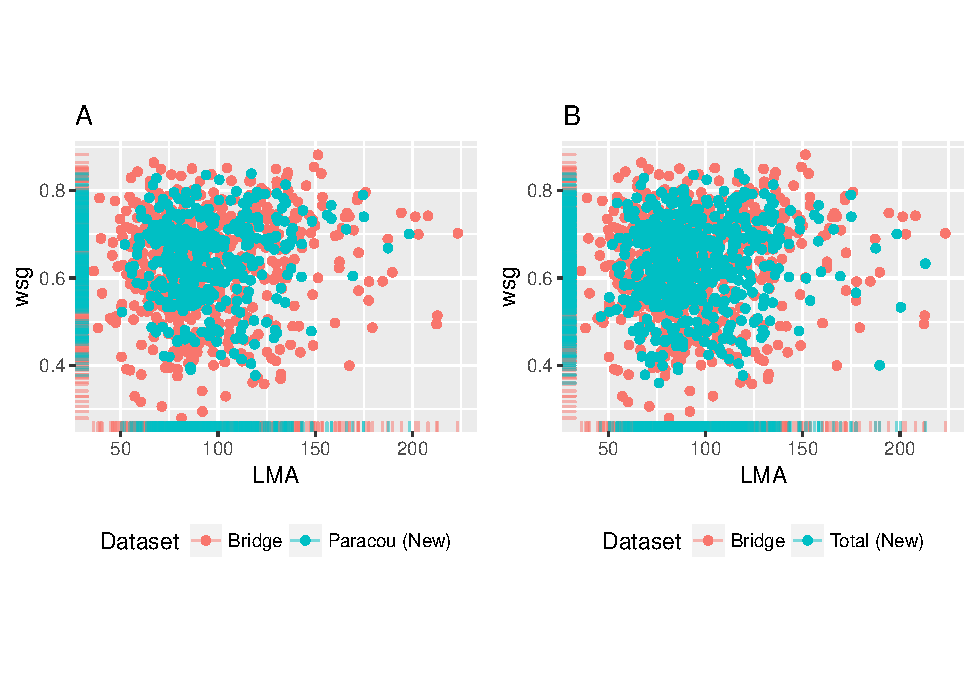
\includegraphics{master-thesis_files/figure-latex/representatfin-1.pdf}
\caption{\label{fig:representatfin} Joint representation of LMA and wsg
distributions for A: the 347 new species set for Paracou, B: the 547
species set used for the selective logging experiment; Compared to the
distribution of the same traits in the total BRIDGE dataset. Colors
indicate whether points belong to bridge (red) or to the inferred
species set (blue). Marginal rugs help to visualise each trait
distribution, and highlight the coverage of their distribution in BRIDGE
(red) by the new species set (blue).}
\end{figure}

\subsection{Discussion}\label{discussion}

In the hierarchical models used here, species means are derived from the
general trait mean. They thus depend on both the number of observations
for each species and the observed trait values. These models allow to
account for uncertainties due to scarce observations: The inferred mean
of a species with few data but extreme trait values is attracted towards
the overall mean, because of high uncertainty due to a low number of
observations. On the contrary, abundant species have narrow confidence
intervals around their deviation to the overall mean; thus a reliably
\emph{distinct} trait mean, even when close to the global mean value.

This is consistent with the idea that using only one measure for a
species is barely more informative than attributing it the community
means, due to sampling stochasticity. Considering the number of rare
species in tropical plant trait databases such as BRIDGE, and given that
each of them contributes to the overall mean, it is arguably to include
them instead of setting an arbitrary cutoff: why would a species mean
computed with five observations more reliable than one computed with
four measurements?

The adjustment of an extreme estimate to a more moderate one is termed
shrinkage and is inherent to many hierarchical models. It can either be
considered an advantageous phenomenon or a problem
\citep[\citet{Mould2013}, \citet{Savic2009}]{Rouder2005}. The main
drawback of this approach is that shrinkage effect leads to an
overestimation of traits distribution densities around the overall mean.
A solution to reduce this bias would be to account for the inferred
distributions of every means: we only used punctual estimations, and
thus ignored a part of the information. This can be enhanced for
subsequent works thanks to a new feature of TROLL, recently implemented
by Fabian Fischer: a species parametrization simulating intraspecific
trait variability constrained by between-trait covariance. This allows
to recreate continuums such as those observed in real forests, by
conserving at least the overall links between every trait.
\citet{Fyllas2014}, for example, used this approach. We could not adapt
our study to this feature, for it was released a few months ago.

\section{Can TROLL simulate real forests and post-logging trajectories
?}\label{can-troll-simulate-real-forests-and-post-logging-trajectories}

\subsection{Overview}\label{overview-1}

The original goal of this section was to evaluate TROLL's aptitude to
simulate post-logging trajectories by using real data. Preliminary
comparison of the model understoreys with seedling and sapling censuses
in Paracou (from the Mariwenn Database), showed that TROLL
underestimates seedling \emph{abundances}, due to discrete space
assumptions (data not shown). It however reliably depicts diameter
structure for higher \(dbh\) categories (\citet{Marechaux2017}). We
compared simulated ecosystem trajectories with regular censuses
(\(>10\ cm\ dbh\)), after adapting the data to the model input format
and simulating the understorey strata. Since the obtained results showed
anomalies, this yielded another question: is TROLL adapted to simulate
forests from real data? We used a spatial statistic approach, comparing
real censuses with mature forests simulated with comparable species
composition.

\subsection{Methods}\label{methods}

\subsubsection{Handling missing species}\label{handling-missing-species}

We used our new species dataset to simulate post-logging trajectories at
Paracou. Overall, 347 Paracou species matched with our dataset,
resulting in higher yet still high proportions of individuals belonging
to missing species. The number of species matching at a plot's scale was
enhanced with the new dataset, but still low (100 to 220), compared to
the 200-350 species that can occur in a single plot
(\ref{fig:newhistrol}. The representativities of these subsets was
overall correct (data not shown). To handle species that were still
missing, we replaced the individuals belonging to missing species by
individuals of parametrized species, by diameter class.

\begin{figure}
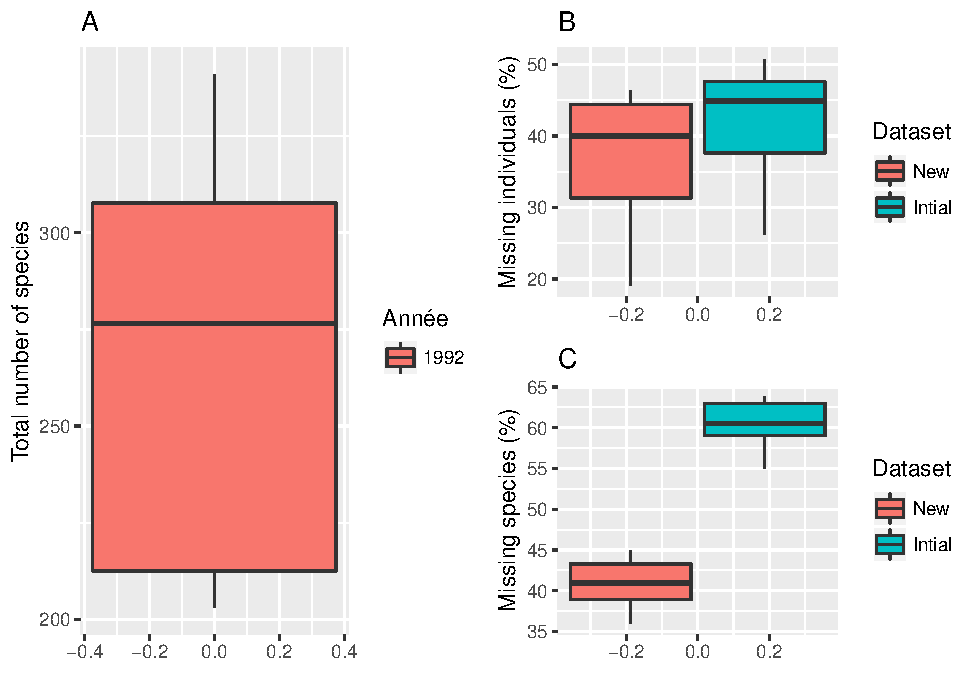
\includegraphics[width=0.7\textwidth]{master-thesis_files/figure-latex/newhistrol-1} \caption{Comparison of the coverage (species and individuals) between the initial and new dataset. A: Total number of species in the plots. B: Proportion of missing (uncovered) individuals. C: Proportion of missing species. Colors indicate the dataset used: blue for the initial set, red for the new one. }\label{fig:newhistrol}
\end{figure}

\subsubsection{Residual mortality after logging: where to start from
?}\label{residual-mortality-after-logging-where-to-start-from}

Residual mortality after selective logging is a well-observed
phenomenon, which has been documented for seven sites in the Amazon
\citep[five in Brazil, one in Suriname, and Paracou - see][ for a
summary table and references]{Blanc2009}. During six to sixteen years
after disturbance, logged stands undergo high persistent mortality which
is due to several factors:

\begin{itemize}
\tightlist
\item
  Many trees are hurt during operations. They do not die immediately,
  but rather a few years after being hurt, especially when poison
  girdling is carried out.
\item
  Soil modifications (compaction, degradation, and ultimately erosion)
  can also stress the trees located near the main or secondary tracks.
\item
  Changes in the abiotic environment due to gap opening can be
  detrimental to some trees.
\end{itemize}

We used Paracou data and Geraldine Derroire's mortality function
(unpublished) to check the annual mortality rates in the 12 plots at
Paracou. Paracou plots have undergone different treatments, consisting
in conventional selective logging (T1), additional Timber Stand
Improvement (TSI - thinning by poison girdling: T2, T3), and additional
fuelwood harvest (T3). Control plots (natural forests, T0) are also
included. The annual mortality rates observed at logged plots to go back
to levels comparable to control plots about ten years after logging
(Figure \ref{fig:mortality} in appendix 5, and see \citet{Blanc2009}),
although there is no neat transition. Still, for treatments 1 to 3, the
mortality levels six years after logging are reasonable compared to
rates observed in the first three years following disturbance.

Considering that 1. the number of botanical indeterminations decreased,
and the ``coverage'' by TROLL species list increased over time at
Paracou; 2. residual mortality decreases between 6 and 8 years after
logging in this dataset; and 3. we want to model as much as possible the
entire trajectory following logging; we started the simulations from
1992, which is an acceptable compromise.

\subsubsection{Coordinates and duplicates: moving, or
removing}\label{coordinates-and-duplicates-moving-or-removing}

Paracou inventories are real forest data at a \(0.5m*0.5m\) resolution,
and TROLL simulates forests with horizontal cell size set to 1m². Other
resolutions are technically possible, but were not further explored, and
increase computation time. As TROLL supports only one tree per cell, we
handled cells containing several trees: the solution was either to keep
only the most prominent tree in each conflicting cell or to replace the
smallest trees in a randomly sampled, nearby free cell with an algorithm
(details available on demand). Both introduce some bias, as it consists
of direct modification of the raw data. Deleting trees is, in our
opinion, worse than moving them of 1 or 2 meters, because it has more
impact on canopy structure, thus on competition for light, which is the
central process modeled with TROLL.

\subsubsection{Missing understoreys}\label{missing-understoreys}

Paracou censuses only include trees over 10 cm dbh, whereas TROLL
simulates trees from 1 cm dbh (or 1m height). Direct similation from
Paracou censuses, without any tree under 10 cm dbh initially present, is
highly erroneous. The regeneration of the understorey strata from
scratch would inducs a latency between the beginning of the simulation
and the first ``recruitment'' events(\emph{sensu} reaching
\(10\ cm\ dbh\)). In reality, recruitment happens continuously and new
trees over \(10\ cm\ dbh\) are registered every year. We thus had to
dodge this problem the most reasonably as can be: We first simulated the
forests' understoreys, that we re-injected in the initial maps.

We considered the following simplifying assumptions:

\begin{itemize}
\tightlist
\item
  To simulate an understorey with TROLL in order to simulate a plot with
  TROLL is than using another solution (for consistency).
\item
  TROLL simulates explicitely competition for ligth, so the
  upper-stratae spatial structure impact the lower-stratae.
\item
  Even if logging damages let part of the \textgreater{}10cm trees
  survive, the understorey must have been more impacted in the
  corresponding areas : skidders and bulldozers tend to avoid big trees,
  but slaughter small trees.
\item
  Thus, the understorey of a logged plot is finally a spatial mixture of
  ``mature state'' and ``early stage'' understoreys.
\end{itemize}

We derived modeling choices considering these assumptions:

\begin{itemize}
\item
  The final understorey we use to inject to the \(>10dbh\) census for
  logged plots is constructed from two distinct TROLL simulations of two
  different censuses, and spatially consistent with the geographic data
  available for the plots and the upper strata structure.
\item
  For undamaged zones in disturbed plots, we simulated the understoreys
  from the last Paracou prelogging census during 30 years, which was a
  compromise between a ``mature state'' understorey and having initial
  (real) trees still alive, for spatial consistency.
\item
  For areas located within damaged zones, we simulated an understorey
  from the 1992 censuses for 5 years, to obtain a young understorey that
  has undergone high enlightenment in opened areas
\item
  For control plots, a single understorey was simulated for 30 years and
  reinjected in the census.
\end{itemize}

We used damaged areas shapefiles obtained from
\url{https://paracoumaps.cirad.fr}.

\subsubsection{Simulation parameters}\label{simulation-parameters}

The simulation parameters were all TROLL default parameters (calibrated
in \citet{Marechaux2017}, adapted for the new version by Fabian Fischer
(\emph{pers. comm.}), except the seedrain scaling constant and the
mortality rate parameters.

We initlally tested a wide range of seedrain parameters to determine the
values that gave realistic results, to use if for our subsequent
\emph{in silico} experiment. This constant can have a strong influence
on commercial tree species regeneration, of which depends directly the
conclusions we can draw from logging experiments. TROLL's default to
simulate forests from bare ground is C\_seedrain = 50000 seeds/ha, and
certainly overestimates the importance of this process in our framework.
We tested 100\%, 50\%, 25\%, 10\% and 5\% of the default value.

Mortality parameters were first let to default values (i.e.~the minimum
mortality rate, m0 = 0.025; and the slope, m1 = 0.025), but we tested
softer mortality rates \emph{a posteriori}, decreasing from 0.020 to
0.010 since the results were highly unrealistic.

\subsubsection{Spatial structure
analysis}\label{spatial-structure-analysis}

After seeing the first outputs, we simulated mature forests
corresponding to each plot in terms of species composition (regional
frequencies set to plot frequencies and default seed-rain scaling
constant). Simulations lasted 600 years, which is assumed to be the time
needed to reach ecosystem maturity in TROLL for high seed-rain constant
values \citep{Marechaux2017}.

Spatial statistical analyses were performed using the ads R-package
\citep{Amap2015}. We compared the spatial structure of TROLL and Paracou
forests using classical spatial indices, based upon Ripley's K function
\citep{Ripley1977}: L(r), a linearization of Ripley's K
\citep{Besag1977}; and g(r), the pair density function;. The first (L)
is linked to the expected number of neighbours present in a circle of
radii r and centered on each point of the map. The second (g) is linked
to the mean number of neighbours present between two consecutive circles
at a distance r and r+dr, for all the points in the map.

\subsection{Results and discussion}\label{results-and-discussion}

\subsubsection{Simulated trajectories}\label{simulated-trajectories}

\begin{figure}
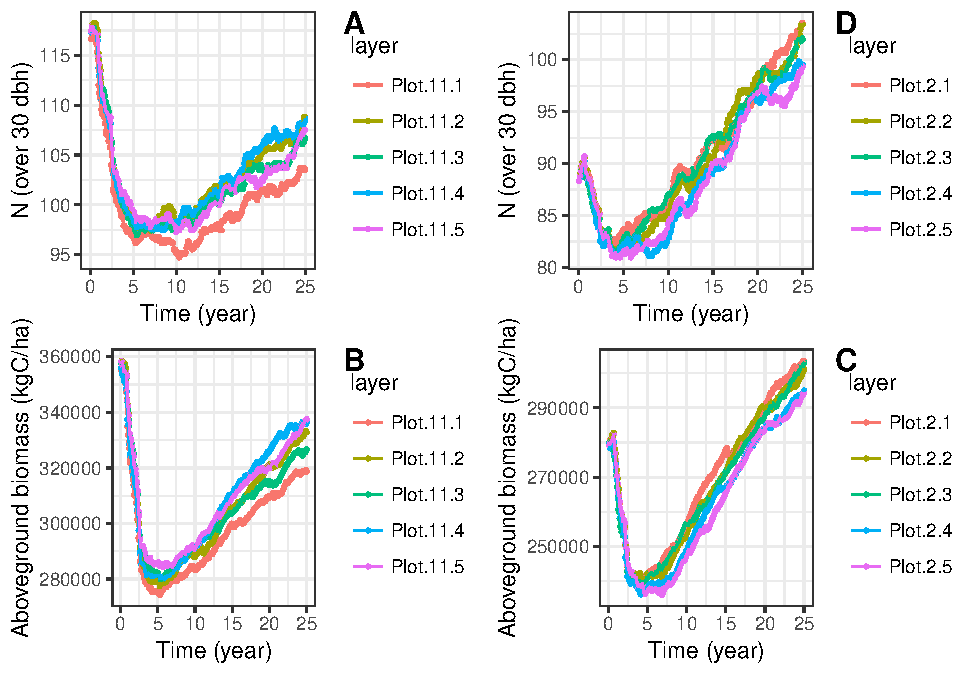
\includegraphics[width=0.8\textwidth]{master-thesis_files/figure-latex/paracoutest-1} \caption{Trajectories obtained with TROLL, using real data as an input. A and B are outputs obtained with the plot number 11 (undisturbed). D and C are the results obtained with plot 2 (selectively logged). A and D show tree density per hectare for individuals above 30 cm dbh over time. B and D display the evolution of above-ground biomass over time. Each curve is a distinct simulation. Simulations lasted 5 years. }\label{fig:paracoutest}
\end{figure}

Figure \ref{fig:paracoutest} shows the trajectories obtained for a
control plot (T0) and a logged plot (T1), in terms of above-ground
carbon biomass (AGB, \(kgC.ha^{-1}\)) and densities of canopy trees
(\(dbh > 30\),N30,\(ha^{-1}\)). In every plot and for every simulation,
we observed an anormal decrease in AGB and N30. This pattern holded at
every mortality rate tested, although high mortality lead to stronger
decreases in AGB and N30. This surprinsing behavior is not likely to be
linked to the way we simulated the understorey, because it affects trees
over 30 dbh. To understand these results, we adopted a spatial analysis
approch, wich results are presented hereafter.

\subsubsection{Spatial statistics}\label{spatial-statistics}

The spatial distribution of trees over 30 cm dbh differed greatly
between real forests (year 1992) and mature simulated forests,
regardless if real plots have been logged or are undisturbed (Figures
\ref{fig:spatialcontrol} and \ref{fig:spatiallogged}). This pattern
holds for every plot (not shown). The \(L(r)\) function (C and D, on
both) curves slightly differ for logged and disturbed plots, with a
slightly overdispersed spatial structure for radii between 3 and 10
meters in control plots. In simulated mature forests, \(L(r)\) reaches
extremely low values for radii up to 10 meters. The rest of the curve
probably stays out of the confidence interval because of the well-known
autocorrelation inherent to \(L(r)\). The \(g(r)\) function curves bring
more reasonable results, yet still showing an stong significant
overdispersion in simulated mature forests, for radii between 1 and 5
meters. The \(g(r)\) curves are computed for consecutive crowns (the
inner-most circle is eliminated). This yields more reasonable,
autocorrelation-free results, yet loosing discrimination power. These
results show that TROLL severely overdisperses trees over 30 cm dbh
compared to real forests at relatively small scale (radius \textless{}
5m).

\textbackslash{}begin\{figure\}
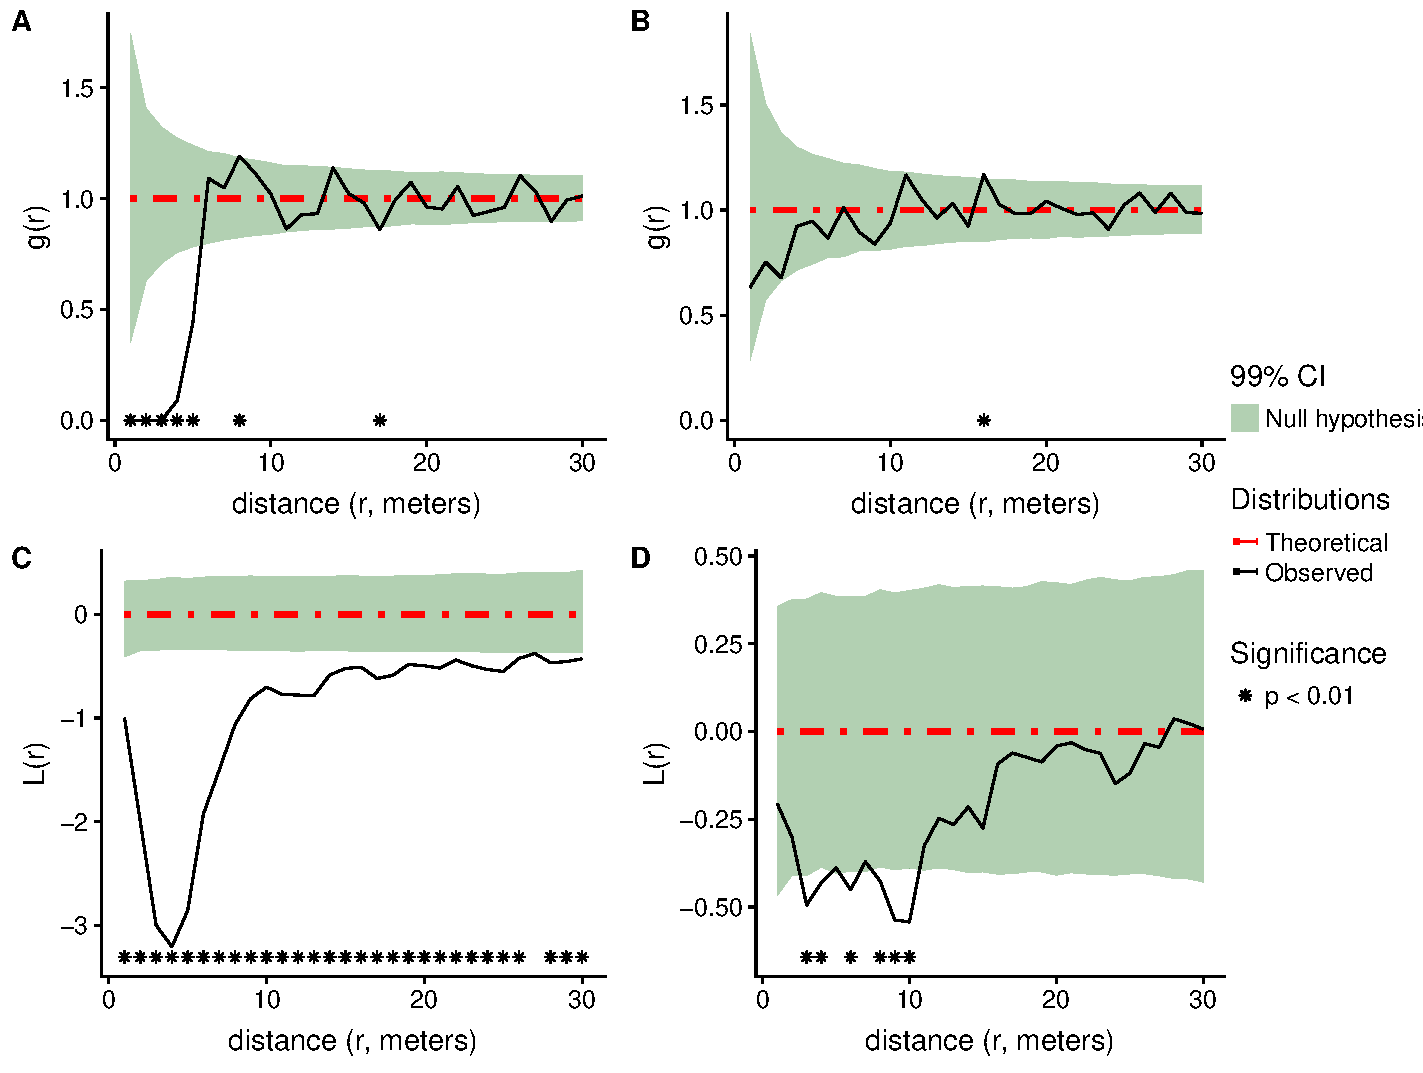
\includegraphics[width=0.8\textwidth]{./plots/p01/Plot_1}
\textbackslash{}caption\{Spatial structure of simulated (A and C) and
real (B and D) forests for Paracou plot P1 (undisturbed). A and B show
the distribution of g(r), the pair density function. C and D show the
distribution or L(r), a linearization of Ripley's K. Both were computed
for 30 radii ranging from 1 to 30 meters. Solid black lines are the
observed distributions, dotted red lines represent the expected mean
distribution under null hypothesis (Complete Spatial Randomness, CSR).
Green areas are 99\% confidence intervals (CIs) around the CSR null
distribution means (for each radius), that were obtained by resampling
randomly trees coordinates (1000 simulations). Parts of the curves that
are out the CIs, for a given radius, violate the assumption of CSR for
this radius. Values under the CIs indicate an overdispersed repartition,
and values over the CIs, a clustered repartition\}\label{fig:spatialcontrol}
\textbackslash{}end\{figure\}

\begin{figure}
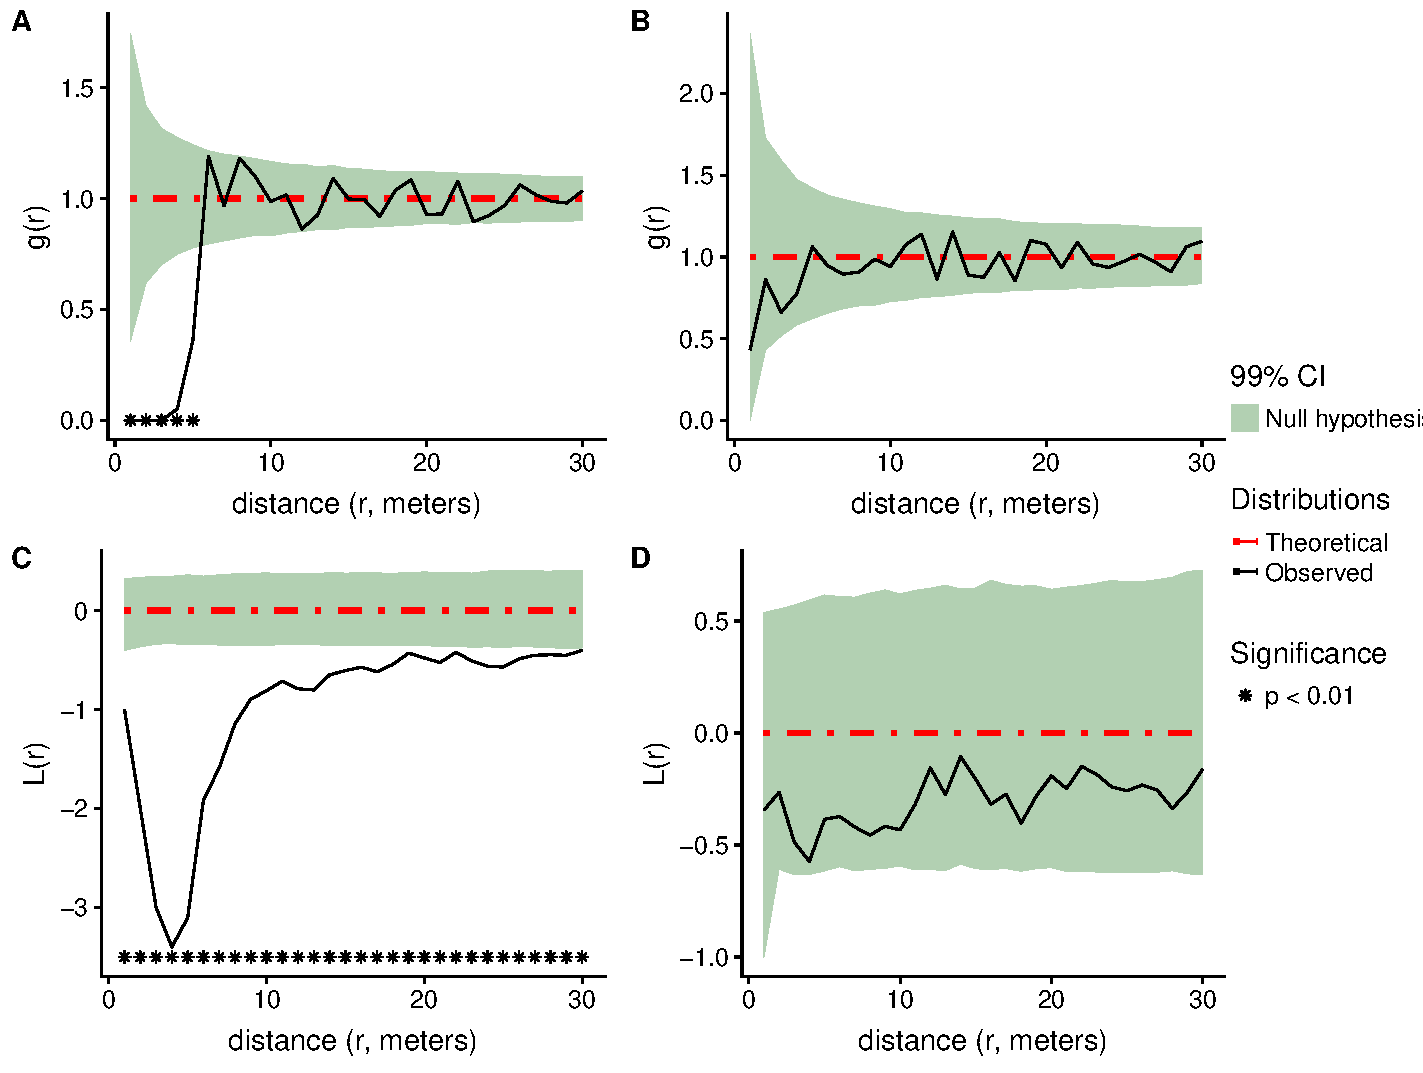
\includegraphics[width=0.8\textwidth]{./plots/p01/Plot_3} \caption{Spatial structure of simulated (A and B) and real (C and D) forests for Paracou plot P1 (logged). These graphics correspond rigourously to the figure, please refer to its label for description and interpretation tips.}\label{fig:spatiallogged}
\end{figure}

\subsubsection{Synthesis}\label{synthesis}

There are several possible reasons to the results of the simulations
from real data. First, it might an inaccurate parametrization of the
model, but \citet{Marechaux2017a} intensively calibrated TROLL. Another
can be an overestimated basal mortality rate, we tested a wide range of
values, and the lowest (0.001) attenuated the phenomenon (not shown).
However, this mortality event was always conspicuously displayed in the
output graphs, for . A factor also influencing the results may be our
data pre-treatment, consisting in replacing trees with duplicated
coordinates. The observed pattern is however homogen for all
simulations, that were led with different random seeds. Our last
hypothesis is that the observed result are due to a difference in
spatial structure between TROLL and real forests, influencing the
modeled light competition effects.

It may seem difficult to disentangle the effects of light competition
and discretisation (cells of 1m²) on TROLL's spatiallisation. We are
comparing two structurally different objects. TROLL is constrained to
homogen spatial structure at fine scale (say, from 1-2 m radius) because
of its assumption of a discrete space, with maximum 1 tree per cell,
while Paracou plots are mapped with a 0.5m resolution. Whilst the same
analysis for saplings or poles (\emph{sensu} \(<10\) and \(<20\) cm dbh)
might only reveal the obvious effects of TROLL's design, focusing on big
trees (over 30cm dbh) brings interesting clues to explain the results
observed with simulations from real data.

Competition for light is the principal ressource-limiting process
modelled in TROLL, which reproduces realistic forests in terms of global
variables and floristic composition \citep[see][]{Marechaux2017}. It
seems likely that TROLL underestimates trees' tolerance to shade or
vicinity with other big trees, thus making simulation from real data
irrelevant for structural reasons.

We can question the validity of the model, because in natural forest,
certain demographic and successional processes rely on trees vicinity,
for example what we can call \emph{substitution}, a successful strategy
some trees, consisting in thriving close to bigger ``pairs'' to benefit
additional water and nutrients (Stéphane Traissac, \emph{pers. comm.}).
However, the fact that TROLL might overestimate competition for light,
and makes forest with overdispersion of big trees, certainly does not
take away its numerous strengths. TROLL is still an valuable tool for
various purposes, such as jointly simulating carbon and biodiversity
(\citet{Marechaux2017}), exploring the impact of forests composition on
ecosystem resilience (\citet{Schmitt2017}), or simulate selective
logging with unequalized spatial resolution. Modelling real forest with
TROLL is just not what it is meant to\ldots{} for now. Future
developments may enable to do it.

\section{Modelling silviculture with TROLL: from reality to
simulations}\label{modelling-silviculture-with-troll-from-reality-to-simulations}

\subsection{Introduction}\label{introduction-2}

To model silviculture in French Guiana with TROLL, we used the first
version of the logging module, which we updated according to
bibliographical infoormation \citep[mostly in][]{Guitet2011} and
numerous communications with Laurent Descroix, head of the RD pole of
the National Forels Office (ONF).

Silvicultural practices \emph{largo sensu} encompass selective logging
with or without cutting cycle, tree plantation, and stand improvement,
such as enrichment planting or tending operations. Nowadays in French
Guiana (FG), silviculture operations mainly consist in selective
logging. Tree plantations are not yet a practice to generate timber
incomes, but promising experiments are ongoing \citep[Project
ForesTreeCulture;][]{Nicolini2016}. Stand improvement often consisted in
thinning by poison-girdling, but this practice has been left apart
\citep{Guitet2011}. Currently, Sylviculture in French Guiana is oriented
towards reduced impact logging (RIL). It is called ``silviculture'' for
the care that is taken in the operations. Part of the aim is to destroy
as less future trees as possible, and optimize natural regeneration
processes by reducing damages and canopy opening during operations.
Notwithstanding these remarks, we mostly refer to ``silvicultural
treatments in FG'' as ``selective logging'' in this whole report.

Selective logging is currently divided into three fundamental parts:
Tree choice, Harvesting. Both encompass different steps and effects:

\begin{itemize}
\tightlist
\item
  Areas and tree choice:

  \begin{itemize}
  \tightlist
  \item
    Definition of the harvestable areas and main track planification
  \item
    Designation of the harvestable trees by the ONF
  \item
    Minor selection from the loggers
  \item
    Tree probing
  \end{itemize}
\item
  Harvesting operations:

  \begin{itemize}
  \tightlist
  \item
    Tree Felling
  \item
    Main tracks opening
  \item
    Secondary tracks opening
  \item
    Bole skidding
  \item
    Post-logging, residual damages
  \end{itemize}
\end{itemize}

Each of these processes is modeled either explicitly or implicitly.
Hereafter, we detail these processes and effects in two parts: * What
currently happens with RIL implementation, or used to with
``conventional'' practices * The way we model the process in TROLL

The modified version of the code will be stored in a public Github
Repository.

\subsection{Choosing area and trees}\label{choosing-area-and-trees}

\subsubsection{Harvestable areas}\label{harvestable-areas}

\paragraph{Reality}\label{reality}

The ONF subdivides forest areas into plots or sampling units. Their
surface area is variable (from 20 to 250 hectares; Laurent Descroix,
unpublished data), but often somewhere between 20 and 50 hectares.
Mechanical and ``floristic'' constrain the choice of harvestable areas.
Bottomlands and swamps are avoided. Steep slopes are also avoided due to
mechanical constraints. Lateral slopes are especially restricting
because they increase the risk of ``sweeping effect'' (when the bole,
tied to a cable, slips laterally) or engine fall, and thus can cause
accidents and considerably increase the damages. Because of such
constraints, sampling units are nearly always located on plateaus or
smooth slopes around hill crests.

In conventional logging, the definition of harvestable areas follows
approximately the same rules. Perhaps the guidelines mentioned above are
not carefully respected as in RIL, because of prevailing profit
interests and untrained crew, but it is as least comparable concerning
human and mechanical safety.

\paragraph{Model}\label{model}

Topography is not yet implemented in TROLL model, which implicitely
assumes a flat environment. Thus, we consider the whole simulated plot
as a harvestable area. We simulated 24 \(ha\) plots (\(400*600\ m^2\)),
thus making a compromise between simulating realistically big plots, and
computational costs.

\subsubsection{Designation}\label{designation}

\paragraph{Reality}\label{reality-1}

Designation was implemented with RIL by the ONF in 2007
\citep{Guitet2011}. It consists in mapping trees and tag trees to be
harvested for the current harvest, future trees to keep for the next
harvest, and ``reserve'' trees (ecologically important, or threatened
species). The designation is made in order to meet the tarvet volume,
and the preference of the loggers: the ONF does not designate trees that
will not be sold. High rank species are ``protected'' by additional
designation rules, that depend on stand spatial structure. For example,
one individual of Dicorynia guianensis is marked as ``reserve'' every
100 meters in large aggregates. This is supposed to let enough
reproductive individuals to ensure the stock in the next rotation. In
CL, there were no designation. The loggers used to choose the trees, and
generally focused on a few species, and big individuals.

\paragraph{Model}\label{model-1}

Designation was deeply modified in the new version of the module. For
consistency with field reality, the designation process is now tailored
to depend the interest loggers have for the different species present on
the plot, in a simple way.

There are a myriad of methods to model choice and preference, and this
is a huge theoretical field of statistics and mathematics
\citep{Kaci2011}. A choice basically depends on which entities that are
confronted, which are the preferences of the actor who choose, and the
presence of other entities or contextual factors.

To model designation oriented by the preferences of loggers for some
timber species, we splitted species into categories and established
simple rules to choose which trees to harvest. In concrete terms, the
categories are interest ranks and the contextual variable is the
individual's diameter. We defined the following relationships inside and
between categories :

\begin{itemize}
\tightlist
\item
  The preference between two individuals of different ranks is direct
  and unvariant. Preference is oriented toward the lowest rank number
  regardless to diameters (provided it matches the minimum cutting
  diameter).
\item
  The preference between equal rank ndividuals depends on their
  diameter. The biggest one is picked, because it yields more timber.
\item
  If diameters and ranks are equal, both can be indifferently be picked.
\end{itemize}

We use three interest ranks in to match the 3 overall categories of
species : * Always harvested and highly demanded (all Principal Major
Commercial Species - ECMP, and \emph{Bagassa guianensis}) * Species
harvested if the first are not abundant enough (most of the Other Major
Commercial Species - ECMA) * Species nearly never harvested, but
sometimes \footnote{In reality, loggers often harvest less than the
  target volume if the stand is not commercially interesting enough, but
  this is not what we wanted to simulate here.} if the two others are
really unsufficiently abundant.

In the model, the relashionships between these categories a fixed. To
simulate harvesting diversification, we made species interest ranks vary
(\emph{cf} next section), but not the way ranks interact with each
other. Our modelling framework is simplified : Additional protection
rules and the ``reserve'' designation are not implemented yet.

\subsubsection{Tree Probing}\label{tree-probing}

\paragraph{RIL and conventional}\label{ril-and-conventional}

Generally, 20\% of the trees matching commercial criteria (species and
diameter) have redhibitory defaults and are considered ``rotten'' by the
lumberman after probing. The causes of these defaults are partially
mysterious. The observed symptoms are generally: the presence of holes
on the trunk or the basis; the break of a big fork that has not
cicatrized; or a hollow sound of the trunk. The probability for a tree
to be rotten depends on its diameter.

The ONF ``encouraged'' the loggers to harvest all trees, including
rotten ones, during an experimental campaign, and gathered data on the
probability to be probed rotten, the actual rotten volume, and the
characteristics of the trees (Laurent Descroix, pers. comm.). According
to this data, around half the designated trees probed rotten by
lumbermen are intact on a \emph{ca.} 90\% of their bole volume. If the
fuelwood demand is expanding during the next years, harvesting rotten
trees may be advantageous. Conversely, these trees may better be let on
the plot, because they can survive and keep producing seeds.

\paragraph{Model}\label{model-2}

We used \citet{Schmitt2017}'s models, calibrated on the mentioned
dataset, to describe the probability for a tree to be rotten, and the
proportion of intact wood in rotten trees. The first is already
implemented in the module :

\begin{equation}
  \begin{array}{c} 
    probbed~rotten \sim \mathcal{B}(P(probbed~rotten)) \\
    P(probbed~rotten) = logit^{-1}(\beta_0 + \beta_1*dbh) = \frac{e^{\beta_0 + \beta_1*dbh}}{1 + e^{\beta_0 + \beta_1*dbh}}
  \end{array}
  \label{eq:rotten}
\end{equation}

The probability for a tree to be \(probbed~rotten\), noted
\(P(probbed~rotten)\), follows a \(Bernoulli\) probability law. The odds
for a tree to be probbed as rotten is the sum of a basal odd
\(\beta_0\), and a diameter dependent odd proportional to \(\beta_1\).
The probability for a tree to be probbed as rotten \(P(probbed~rotten)\)
is the inverse logit (\(logit^{-1}\)) of the odd (see
\citet{Schmitt2017} for the detailed model design).

We implemented the rotten volume model as well, to compute the volume of
energy wood potentially valuable from rotten trees, given by:

\(V_{intact} = 8.9dbh^2(1-(0.4*dbh^2))\)

\subsection{Then, harvesting}\label{then-harvesting}

\subsubsection{Felling trees}\label{felling-trees}

\paragraph{Reality}\label{reality-2}

In RIL, directional felling is theoretically implemented to avoid
damaging leave (``reserve'') trees. The basic treefall direction is
considered random, but in fact depends on the trees' natural orientation
and crown aspect. Oriented treefall aims at orienting logs at \emph{ca}
\(30^{\circ}\) in relation to the track (main or secondary), to reduce
damages when skidding and to handle the logs more easily. Unfortunately
few harvesters currently apply this technique in French Guiana, at least
for now. Its implementation is ongoing, being part of the ONF's goals.

In conventional logging, few care is taken in felling the trees. The
orientation is not controlled, and future trees are not accounted for at
all. It makes it more dangerous for workers, and the damages in the
understorey are expected to be higher.

\paragraph{Model}\label{model-3}

The complexity and computational costs involved with directional felling
implementation are too high regarding the gain that it represents. A
fully functional oriented treefall function would do it by assessing,
for each harvested tree, what orientation fits with the closest track
and involves the minimum damage for future merchantable trees, which
would have to be preliminarily marked. We hope that further developments
of the module will bring an easy and computationally efficient way to
implement this feature. In the current implementation, trees are felled
at random angle, and gap dimensions are kept in memory to subsequently
compute post-logging damages.

\subsubsection{Main Track}\label{main-track}

\paragraph{Reality}\label{reality-3}

Foresty roads and tracks are split in three categories: truck roads,
main tractor track, and secondary track (\emph{cloisonnement}). In each
plot, the main track is designed following the crest line (using digital
elevation models). The main track extent within the sampling unit
generally depends on the quantity of wood available in the plot. If more
than 100 cubic meters of wood are transiting on a segment of forest
track, the main track must be built up to there, probably to avoid
excessive damages to the soil (that cause compaction, erosion and
ultimately, infrastructure destruction). Wood quantity can be assessed
directly, or using using surface as a proxy. This second option is often
used, but assumes an isotropic distribution of harvestable trees, which
is often violated to some extent.

\paragraph{Model}\label{model-4}

Given TROLL's assumption of a flat environment, the main track is opened
from the midle of one side of the plots with a width of 6 meters, and
traced untill reaching the point corresponding to a volume threshold.
The extent of the main track is foreseen using the targetted volume and
the dimensions of the plot, and the surface uncovered by the main track
correspond to the volume threshold, approximately. We choosed to use a
threshold of 250 \(m^3\), instead of the 100 \(m^3\) used by the ONF.
This adaptation was specific to the size and shapes of our plots, and is
partly wrong. However, with 100m3, the main track always reached very
close to the other edge of the plot, and this was conceptually
disturbing.

\subsubsection{Secondary tracks}\label{secondary-tracks}

\paragraph{Reality}\label{reality-4}

A major improvement in RIL is the mapping of felled trees and the usage
of topographical relevés to optimize the secondary tracks network. The
National forest office currently uses these tools to trace manually the
secondary tracks in a way that more wood is extracted for a reduced
track area. Software developed by the CIRAD and ONF is also used to
optimize the tracks automatically but is currently still improved, to
become fully functional. Recent improvements, such as the use of a nylon
cable to skid the logs, also allow reducing the damage, because the
tracks do not have to go up to every tree. Thus, tracks are designed to
go between trees, approaching them to a distance of 30 meters maximum.

Conventional logging was primarily characterized by the absence of GPS
mapping and topographical relevés. Skidding tracks were designed
directly in the field. Thus, some trees were omitted and the track
network used to be everything but optimal. There is no evident way to
describe how tracks were typically traced. Bulldozers were used to go up
to every felled tree, following the (somewhat imprecise) approximations
of lumbermen. Overall, this could be more related to sight-based
skidding, and getting trees from close to close.

\paragraph{Model}\label{model-5}

We modeled both conventional and RIL skidding fashions. RIL skidding was
already implemented in the first version of the modules
\citep[see][]{Schmitt2017}. CL was modeled using the simple assumption
that the closest tree is first harvested, and the next ones, from close
to close.Figure \ref{fig:tracksRIL} shows maps generated with both
options, at two different harvest intensities. Note the difference in
track extent, and the dependence to target volume.

\begin{figure}
\centering
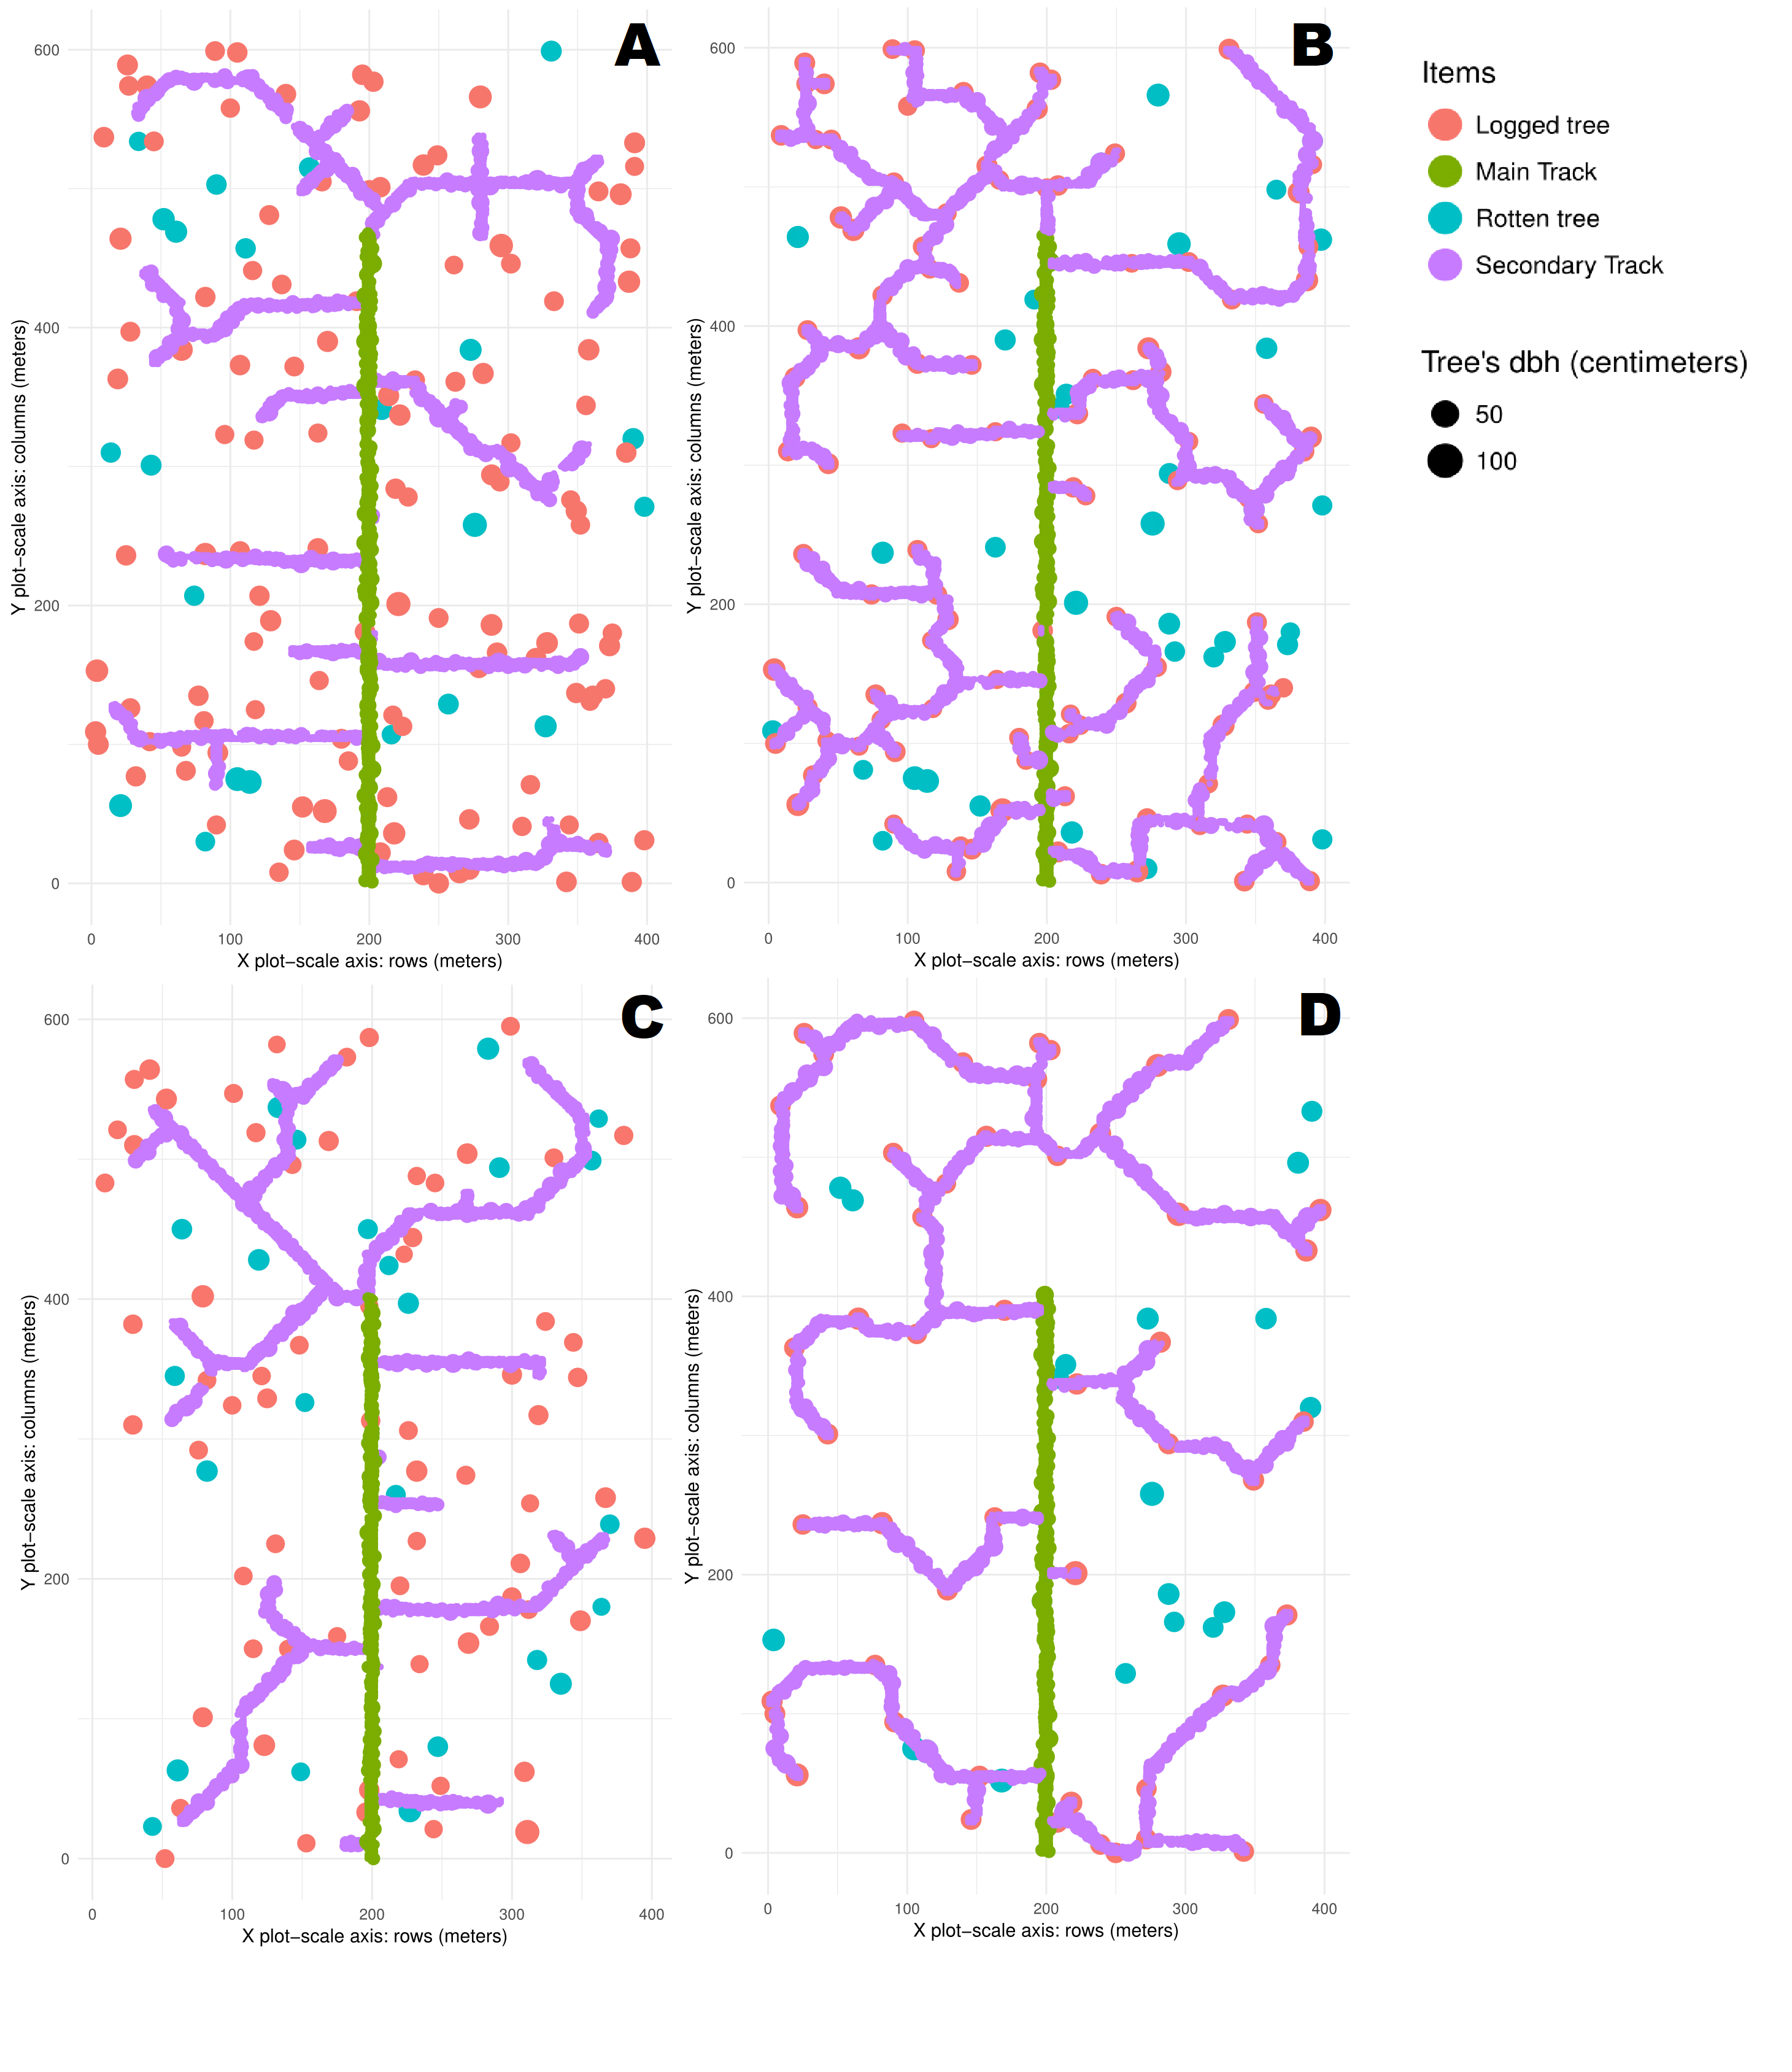
\includegraphics{images/logging_fig.png}
\caption{\label{fig:tracksRIL}Maps generated by the selective logging
module. A and B are maps obtained with a target volume of 30 cubic
meters. For C and D, target volumes were 20 cubic meters. A and C were
simulated with the RIL configuration. B and D were simulated with the
conventional logging configuration.}
\end{figure}

\subsubsection{Residual mortality}\label{residual-mortality}

\paragraph{Reality}\label{reality-5}

Logging operations have immediate and secondary damages on tree stands.
Secondary damages are way less conspicuous than immediate damages and
cause residual mortality during the first years after logging. These
damages can be due to direct hurts of the remaining trees during felling
or skidding (uprooted stems, stem wounds, and bark scrapes), or due to
the induced habitat changes. As exposed in section 4 of the thesis,
mortality rates are higher at Paracou during the first years following
logging, from 1987 to 1994.

\paragraph{Model}\label{model-6}

Generally, long term damages due to selective logging are modelled with
a 10 years increased mortality \citep{Huth2004, Khler2004, Ruger2008}.
We used the model developed by \citet{Schmitt2017} last year, who
gathered data from Paracou censuses between 1988 and 1992 on harvested
plots and adapted the model from \citet{Herault2010} based on a
disturbance index into:

\begin{equation}
  \begin{array}{c} 
    Death \sim \mathcal{B}(P(Death)) \\
    P(Death) = logit^{-1}(\theta + \beta*e^{\alpha*d_{gaps}}) = \frac{e^{\theta + \beta*e^{\alpha*d_{gaps}}}}{1 + e^{\theta + \beta*e^{\alpha*d_{gaps}}}}
  \end{array}
  \label{eq:death}
\end{equation}

\(Death\) of a tree follows a \(\mathcal{B}ernoulli\) law of probability
\(P(Death)\). The odds for a tree to die are calculated with the sum of
the natural tree death odd \(\theta\) and a perturbation index
\(\beta*e^{\alpha*d_{gaps}}\). The perturbation index depend on the
distance \(d_{gaps}\) of the tree \(i\) to the closest logging gap. The
probability for a tree to die \(P(Death)\) is finally calculated by
taking the inverse logit \(logit^{-1}\) of the odd.

\section{Selective Logging
experiment}\label{selective-logging-experiment}

\subsection{Experiment design}\label{experiment-design}

In French Guiana, 77\% of carbon emissions would be due to deforestation
and selective logging would account for 5\% of these emissions, although
uncertainties are high \citep{Cabon2015}. Nowadays, about 80 000 m3 of
wood are harvested by selective logging each year in French Guiana. This
quantity slowly increases year by year. Current demographic growth in
French Guyana is at a level which arguably can lean to a double increase
of the population by 2030. Given this estimate, and a general aim to
develop wood industry (the only possibly sustainable lucrative activity
in French Guiana, opposed to gold mining), current projections aim at
200 000m3 of timber harvested per year, to be reached by 2025, along
with a substantial quantity of fuelwood to supply biomass-fueled power
station. This involves either an increased need to designate areas for
logging, or an increase in harvest intensities.

The fuelwood supply is a problematic of growing interest in the region.
Three solutions could answer the increasing demand of wood for energy
supply : * Valorize the wastes that are usually left on the ground
during timber extraction * Dedicate plots for this particular activity *
Take advantage of plantation wood and local species to minimize pressure
on natural forests.

The implementation of fuelwood outputs in TROLL was motivated by this
need, because the quantities that can be obtained from logging wastes
are still uncertain.

\subsubsection{Simulated forests}\label{simulated-forests}

\subsubsection{Diversification of the harvested
species}\label{diversification-of-the-harvested-species}

The choice of harvested trees is essential to allow for regrowth of
merchantable timber species instead of pioneer trees. The
diversification of harvested species has long been proposed as a
solution to mitigate the adverse demographic impacts of logging of these
species \citep{Guitet2011}.

In French Guiana, more than 100 tree species are recognized for their
technological qualities, and are referred to as commercial species.
However, only a handful of species constitute the majority the overall
extracted timber volume \citep[every information on timber species is
in][]{Guitet2011}. Commercial species are classified according to 4
categories: * Principal Major Commercial Timbers (ECMP) * Other Major
Commercial Timbers (ECMA) * Precious Timbers (BP) * Other Commercial
Timbers (AEC) Currently, only every ECMPs and one ECMA (\emph{Bagassa
guianensis}) are subject to designation to be harvested. One the one
hand, the ONF insist on the need to diversify the set of harvested
species, without what current choices can only lead to ressource
depletion within a few cutting cycles. On the other hand, they have to
collaborate with logging companies to ensure the operations economical
viability, which is impossible if too much non-demanded timbers, that
can't be sold in the current market context, are designated.

We simulated three situations of preferences starting from the actual
preferences to ideal, total diversification, resulting in three cases
which we refer to as ``realistic'', ``intermediate'' and ``diverse''.
Diversification is modelled with a species-specific interest variable,
and our 3 modalities correspond to three cases:

\begin{itemize}
\tightlist
\item
  Species interest are split into three rank levels :
\item
  1: the few species that are overharvested in reality
\item
  2: species that are occasionally harvested as a complement of the
  firsts
\item
  3: species that are generally avoided, \emph{i.e.} the majority.
\item
  Species interest are split into two rank levels
\item
  1: the previous first and second categories, i.e.~the diversification
  occurs on the species that loggers currently accept only.
\item
  2: the often-avoided species set
\item
  Every commercial species have the same rank
\item
  This is the ideal diversification, the case where every technically
  usable species would be valorised.
\end{itemize}

\subsubsection{Silvicultural parameters}\label{silvicultural-parameters}

\paragraph{Both types of selective
logging}\label{both-types-of-selective-logging}

We simulated both Reduced Impact Logging and ``improved'' conventional
logging, as implemented in the new version of the silviculture module.
The reason of this choice is that both logging types can still happen in
French Guiana: logging companies undergo a rapid turnover, and the
degree of collaboration with the ONF is not constantly ideal. Careless
operations, yet supposed to follow EFI guidelines, can lead to
unoptimized skidding tracks opening and be, in terms of damages,
relatable to conventional logging (Laurent Descroix, pers. com.).

\paragraph{Target and designated
volumes}\label{target-and-designated-volumes}

Current harvests in French Guiana target timber volumes of 25m3 per
hectare in average, and the actual quantity of wood that is extracted is
generally around 20 m3 due to rotten trees that are not yet valorised.
This can however have advantages, such as conserving carbon stocks and
seeding trees.

In the present regional and international contexts, harvest intensity is
a central element of forest management, and can be influenced by two
adverse forces: human needs or ecological concern. A growing body of
evidence suggests that harvests must be regulated at low intensities, to
make selective logging less harmful to the ecosystem. However, in a
region such as French Guiana, experiencing high demographic growth and
with ambitions relative to timber valorisation, there is a pressure to
either uprise logging intensities, or log more forest areas.

We thus tested two target harvesting intensities:

\begin{itemize}
\tightlist
\item
  20 \(m^3\), which is in agreement with the current practices
\item
  30 \(m^3\), which may be a future target according to GFClim scenarii
\end{itemize}

Since the overall proportion of rotten trees is about one third of the
total designated trees, we parametrized the module accounting for this.
The total designated volumes thus were uprisen to 30 and 45 \(m^3\), to
obtain the target volume at the first rotation, in average.

\paragraph{Cutting cycles}\label{cutting-cycles}

The cutting cycle duration is equally a key parameter in sustainable
management. It varies widely in the Tropics depending on the continent,
region, or even the country. In the Amazon, most of the cutting cycles
are currently between 30 and 45 years. French Guiana is an exception,
with cutting cycles fixed at 65 years for the moment. This exception is
thought to be the minimum time that should elapse between two cutting
operations, but this is often inadequate considering economic and
development purposes. This situation may change in French Guiana
someday, if logging is to be intensified in the region.

We tested two durations for a complete cutting cycle: 35 years, which is
the duration that matches most current practices in neighboring
countries (for example Brasil); and 65 years, the choice currently
adopted by the ONF in French Guiana. To assess the alleged
sustainability of such cutting cycles, we simulated logging operations,
and stopped the simulations just before the sixth. This resulted in 175
years of simulation for the short cycle, and 325 years for the long one.

\paragraph{Seed-rain scaling: personal
choices}\label{seed-rain-scaling-personal-choices}

Most of tree species rely on animal pollinators and dispersers to
perpetuate their lineage. Selective logging has adverse effects on these
animals \citep{Kormos2012}. The remaining reproductive adult trees are
probably the major dispersers of seeds in logged plots. Since
regeneration processes and timber species autecology remain mysterious,
the way we model seed dispersion has an impact on the simulation
outcome.

The default value of the seed-rain scaling constant -used in TROLL to
model external seed arrival- overestimates the actual regeneration
potential in the case of logged forests. It is not adapted to simulate
regeneration from logged forests, in which we assume a more enclosed
demographic functioning.

Moreover, in our experiment, we assume that our simulated logged plots
are surrounded by equally logged plots, that thus cannot supply a high
number of seeds to neighboring areas. Thus, we believe that it would be
safer to underestimate the seedrain than overestimate it. We set TROLL's
seed-rain constant on an arbitrary 5\% of its value (2500
seeds/ha/mmonth)

\paragraph{Replication of the
experiment}\label{replication-of-the-experiment}

The experiment is constrained by time and high computational costs. The
present experiment design already yields a total of 48 factor
combinations. We replicated each simulation 5 times with a distinct
random seed, resulting in 240 simulations.

\subsection{Results}\label{results}

\subsubsection{Model features}\label{model-features}

\begin{figure}
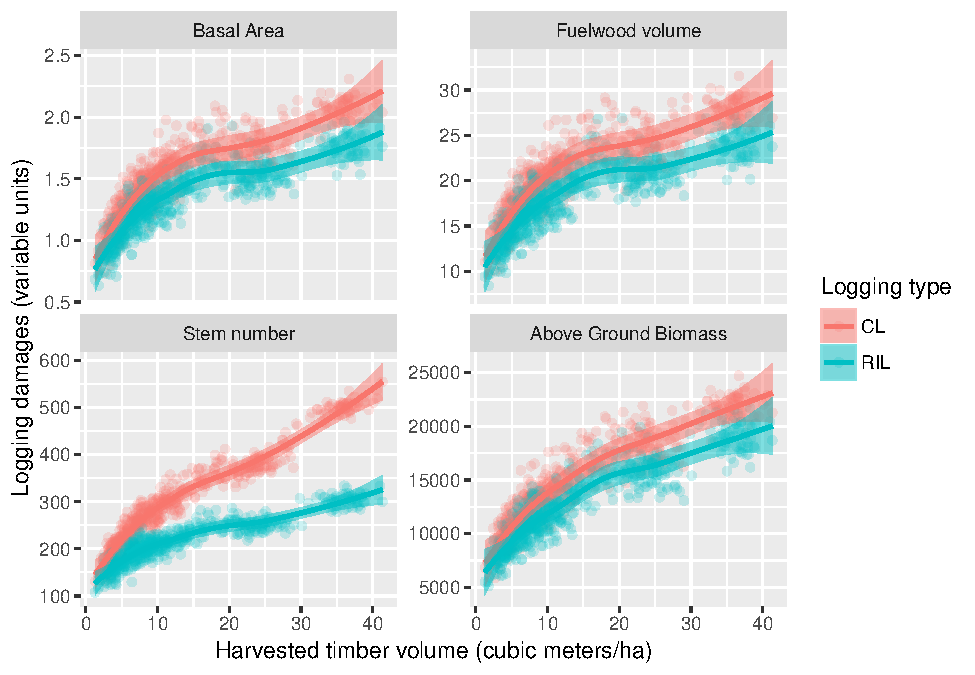
\includegraphics[width=0.7\textwidth]{master-thesis_files/figure-latex/disturbance-1} \caption{Summary of the logging damages caused by main and secondary tracks opening in our simulations (logged and rotten trees are excluded), plotted against the corresponding actual harvested timber volume: removed Basal area (m²), damaged stem count, removed Above Ground Biomass (kgC/ha), and Fuelwood volume (the volume of damaged trees over 20cm dbh). In the model, every damaged tree is at every cutting cycle. Points are all the observations for every scenario tested and all cutting cycles (1200 observations: 240 simulations - 2 forests, 2 target volumes, 2 cutting cycles, 3 designation modes, and 2 logging techniques; with 5 replicated each).}\label{fig:disturbance}
\end{figure}

Unsurprisingly, conventional logging (CL) always caused significantly
higher tracks damages than reduced impact logging (RIL), be it in terms
of above-ground biomass, basal area or stem number (Figure
\ref{fig:disturbance}). The most discriminant indicator, for the two
logging techniques, is the number of damaged stems (over 1 cm dbh),
which is equally unsurprinsing because it is an excellent proxy of the
tracks area\footnote{The maps shown in the precedent chapter are
  actually made with the coordinates of destroyed stems, for which the
  cause of the death is registered.}, that strongly differ between CL
and RIL. For BA and AGB, the difference between CL and RIL is less
pronounced. Each of the four variables is strongly related to the actual
harvested timber volume. Including logged trees makes this relationship
tightly linear, within the range of our harvested volumes, for BA and
AGB. Averaging the whole simulated dataset, we noticed that about one
third of damaged trees died due to the main tracks, and another third
due to secondary tracks. The differences observed between both logging
types are more strongly related to secondary tracks, because the main
track length only depends on the target volume, in our model.
Additionally, the absence of replication of the experiment on several
other initial forests, simulated with different random seeds, may be a
source of biais in estimating main track damages for the first cutting
cycles (after which regeneration occurr at random): it is traced at the
same place on the map for every simulation,with only variations of
length according to target volumes. Thus, differences between CL and RIL
might be more marked if examined on a bigger set of simulations

\subsubsection{Selective logging
sustainability}\label{selective-logging-sustainability}

\begin{figure}
\centering
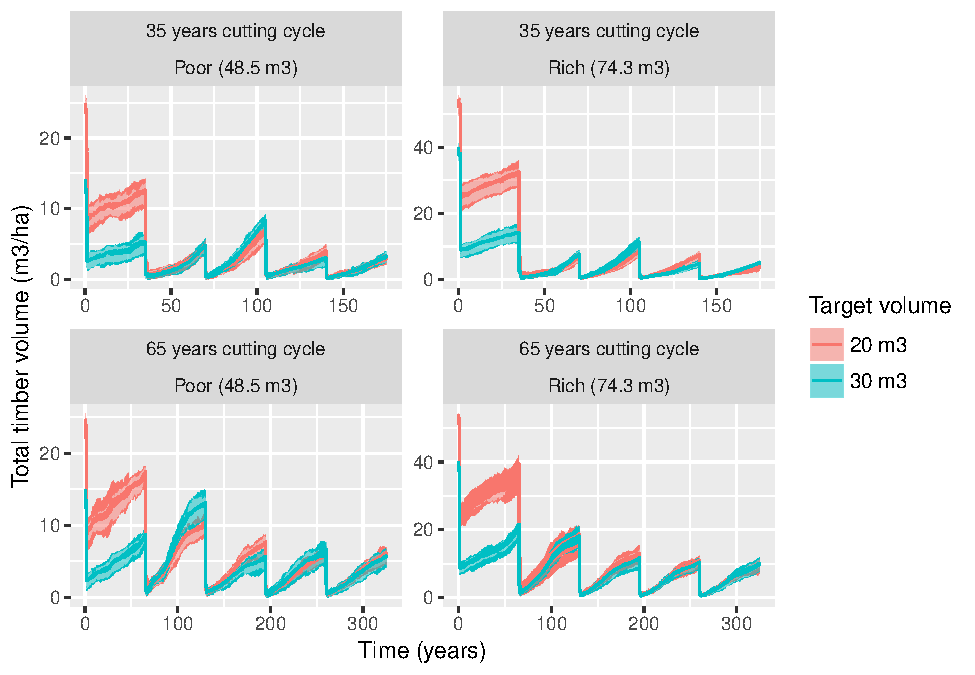
\includegraphics{master-thesis_files/figure-latex/totalvolumes-1.pdf}
\caption{\label{fig:totalvolumes}Simulated evolution of the timber stocks
over 5 complete cutting cycles, for two contrasted (rich and poor)
initial forests -in terms of initial timber stock, cf.~the facets
labels-, with cutting cycles of 35 and 65 years, and target volumes of
20 (red) and 30 (blue) cubic meters. Lines represent the mean trajectory
of 30 simulatons each, and color bands, confidence intervals delimited
by the 1st and 99th percentile computed for the 30 observations at each
timestep.}
\end{figure}

Conventional and reduced impact logging only had a marginal impact on
wood quantity (not shown), probably due to the high harvest intensities
in our simulations. Thus, we pooled these simulations and decided to
emphasize on cutting cycle, target volume, and initial forests.

Our two simulated forests started from 48.5m3 or 74.3 m3 of harvestable
timber. This initial difference did not have a significant effect on the
final outcome over 5 rotations. Total timber volumes importantly
decrease over harvests. The volumes available before the second harvest
strongly differ according to target volumes, and initial timber stocks:
they are higher in the initially rich fores for the lowest harvest
intensity. Cutting cycle length have a marginal influence on timber
volumes for the second rotation. Likely, the initially present and uncut
trees are logged at the second harvest. Trajectories seem to be stable
after 3 of 4 cutting cycles. From there onwards, timber volumes
available at harvest time barely reach 5 and 10 \(m^3\) for 35 and 65
years cutting cycles, respectively.

\subsubsection{Diversification}\label{diversification}

Diversification was simulated by making vary the equitability of
interest ranks for merchantable species. Figure
\ref{fig:diversification} shows the merchantable volume for ECMPs, which
are the actual most valuable timbers. The relaxation of the loggers'
preferences has nearly no effect on the proportion of ECMP
(\ref{fig:diversification}), that decreases, probably because of high
harvested volume. In each case, the proportion of this category of
commercial timbers (the most valued) sinks drastically over rotations.
In our forests, the majority of the timber species (in term of volume)
initially belong to this category, but we simulated a weak external
seed-rain, thus letting the regeneration be more influenced by trees
that are in the plot.

\begin{figure}
\centering
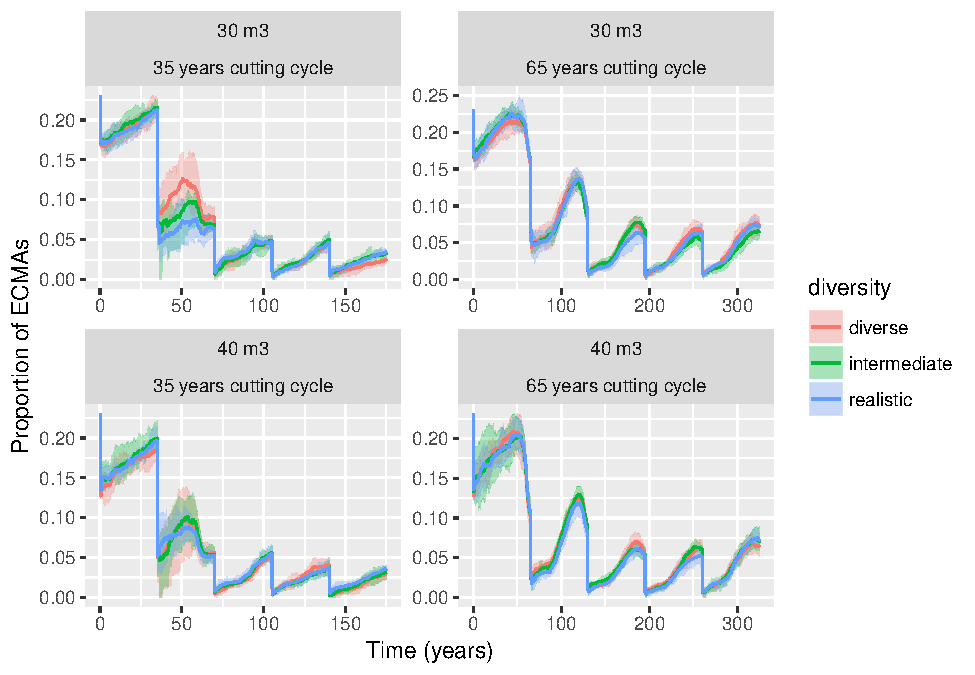
\includegraphics{master-thesis_files/figure-latex/diversification-1.pdf}
\caption{\label{fig:diversification}Total proportion of the merchantable
volume (trees over 55 cm dbh) for Major Principal Commercial Timber
species (ECMPs) over time (years). Diversity corresponds to our 3
designation choice scenarii: Diverse - all species have equal interests;
Intermediate - ECMP and ECMAs are preferred over BPs and AEC; Realistic
- ECMPs are preferred over every other categories, ECMAs are preferred
over BPs and AECs. Color bands are confidence intervals obtained by
pooling replicates}
\end{figure}

\subsubsection{Carbon}\label{carbon}

\begin{figure}
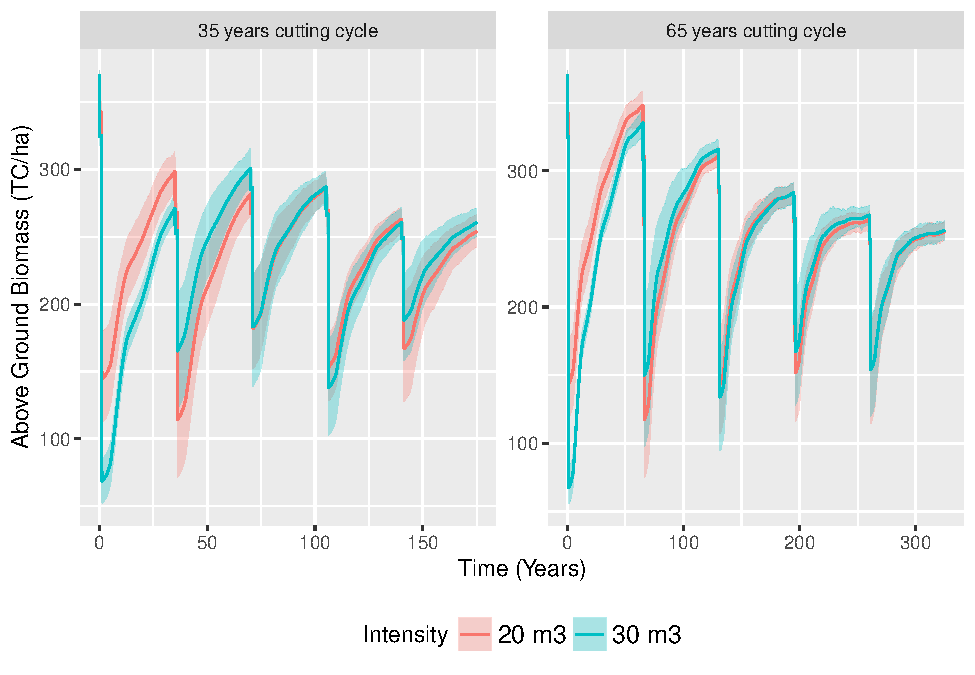
\includegraphics[width=0.7\textwidth]{master-thesis_files/figure-latex/carbon-1} \caption{Simulated effects of selective logging on Ecosystem carbon stocks over time with 5 complete cutting cycles. Simulations are pooled to focus on two keys variables - Cutting cycle, and target volume.}\label{fig:carbon}
\end{figure}

Logging, and post-logging mortality applied one year post-harvest, cause
considerable loss in AGG in any case. For both cutting cycle durations,
the regain in AGB is significantly higher for plot logged at the lower
intensity (20\(m^3\)). After the second cut, intensively harvested plots
seem to regrow their AGB stock faster than less severly logged ones,
once again for both cycles duration, yet this effect is of unlikely to
be significant. From the third harvest onwards, the differences in
harvest intensity is insufficient to change the ecosystem fate: both
trajectories converge towards a maximum value of 250 \(TC/ha\) at the
very end of the last cutting cycle, \emph{i.e.} around 30\(\%\) less
than the original \emph{ca.} 350 \(TC/ha\). The carbon loss is more
progressive for plots harvested each 65 years than those cut every 35
years. The last regrowths, for both, seem likely to stabilize AGB at a
lower level than the initial 350 \(TC/ha\), althought longer regrowth
simulation would be needed to confirm this trend.

\subsection{Discussion}\label{discussion-1}

\subsubsection{Timber volumes are not
sustained}\label{timber-volumes-are-not-sustained}

Our \emph{preliminary} results indicate that selective logging, as
currently carried out, is unsustainable in terms of timber yields.
Ecosystem fates were similar in that every treatment led to a depletion
of timber stocks. Short cutting cycles considerably accelerate this
phenomenon. All factors contribute to the available wood volume at the
\textbf{second} harvest. However, this quantity is best explained by the
initial timber stocks and the target volume than by the length of the
cutting cycles. This dependence on the initial conditions is explained
by unsufficient regeneration of timber stocks, that fails to compensate
for the harvest intensities we simulated. At the second cut, plots were
left with no remaining timber stock in every scenarii. Diversification
of the harvested species had a low impact on the stock of first grade
timbers, which reduced over years in any case. This is probably due to
high harvest intensities. Moreover, elementary protection rules are
currently applied in the field to protect seeding trees for valuable
timbers \citep{Guitet2011}. We did not include it in our model. Our
preliminary results match previous findings from simulation studies. In
his most optimistic scenarios, \citet{Sist2007} predicted a recovery of
50\(\%\) the initial timber stocks at the second harvest for 30 years
cycles, starting from an intensity of \(20 m^3/ha\). They also estimated
an average 10-14 \(m^3/h\) for available timber after 40 years of
regrowth. \citet{Dauber2005} estimated that 4 to 28\(\%\) the initial
total timber volume is recovered before the second cycle, with similar
intensities and duration to those we simulated. In a case study on
\emph{Dicorynia guianensis}, by far the most harvested timber species in
French Guiana, \citet{Gourlet-Fleury2005a} estimated a maximum 60\(\%\)
of volume recovered in any case they tested. \citet{Valle2007} presented
more optimistic results, estimating to 30-40 and 60 years the time
needed to recover commercial volumes for CL and RIL, with similar
intensities. They however concluded that selective logging is
unsustainable without adapted silvicultural treatments.

\subsubsection{Carbon stocks decrease}\label{carbon-stocks-decrease}

Simulated forests undergo a spectacular above-ground biomass (AGB) loss
because of logging and the simulated post-logging mortality. It is
difficult to estimate if this effect is overestimated or not: in
reality, logging damages do not cause an immediate decrease in AGB, but
rather yields extra mortality for several years, less visible because
buffered by regrowth \citep[see][]{Piponiot2016}. In our model,
post-logging mortality is simulated 1 year after logging, and integrates
damages for a 10-year period. This should be revised in the next version
of the model. The total AGB globally decreases over time and harvests
(\ref{fig:carbon}), and the AGB recovery is decelerating after each
harvest. This may be due to a shift in community composition from
shade-tolerant, slow growing tree species to heliophilous, fast growing
stands. \citet{Huth2003}, as well as \citet{Valle2007} observed this
effect in their own simulations. We did not study the evolution in
species composition and diversity, but this shift is likely to happen,
because we simulated low external seed incomes. Thus, we gave more
importance to the surviving trees for reproduction, which seems more
reasonable than a constant, huge arrival of seeds in the plot. However,
our simulations indicate that AGB stocks are partly retained, and
recover faster than other attribute, consistently with other authors
findings \citep{Rutishauser2015}. \citet{Sist2015} suggested that AGB
can be fully recovered 125 after logging, but they did not assess the
effect of multiple harvests.

\subsubsection{In a nutshell}\label{in-a-nutshell}

Our preliminary simulations indicate that selective logging may be
unsustainable in many aspects. Current practices may allow neither to
sustain overall timber stocks nor high value timber yields, nor
fundamental services such as holding carbon stocks. Current cutting
cycles are too short, even in French Guiana, to allow for sufficient
timber species recovery. Harvested volumes are too high, and guarantee
substantial decrease in commercial trees that are not compensated by
remaining trees growth, recruitment, and external seed incomes. However,
our results lack replication and may been interpreted with precaution.

\section{Conclusions and
perspectives}\label{conclusions-and-perspectives}

We inferred seven traits means for 547 species, resulting in better
coverage of Paracou species, needed to address our goals. Post-logging
trajectories were not reproducible starting from real censuses because
of abnormally high mortality during the five first years of simulation.
We hypothesized that this could be related to the model's structure and
assumptions. We verified this hypothesis using spatial statistics and
found an overdispersion of canopy trees (\textgreater{}30 cm dbh) in
TROLL, not observed in real data. Our results indicate that calibration
of post-logging recovery with TROLL requires another approach than
inputting real data into the model. We implemented new generic
functionalities to simulate selective logging in two different ways (CL
and RIL) and test variations of essential silviculture parameters such
as cutting cycle duration, target volume, minimum cutting diameters, and
preferences among timber species. This enables to investigate a wide
range of scenarios with TROLL.

Finally, we did a preliminary set of simulations, testing 24 scenarios
in two different forests. Preliminary results indicate that ecosystem
damages are both sensitive to the target volumes, and the logging
techniques used. In the model, the gain of RIL regarding damages is
mitigated by high harvest intensities. Every scenario we tested to
similar long-term trajectories. Current cutting cycles seem inadequate
with Sustainable Forest Management, no matter what exactly one wants to
sustain: carbon stocks and timber volumes undergo a long-term decreased
in our simulations. Above-ground biomass trajectories are consistent
with forest secondarisation. We did not test the impact of logging on
species diversity and composition in the long term, but it is likely
that pioneer species take advantage of the repeated disturbances caused
by multiple harvests. The majority of the extractible fuelwood volume,
over two rotations, concern trees damages during secondary tracks
opening. The results suggest that TROLL could be useful to explore
scenarios and provide first estimates of the quantity of fuelwood that
could be valorized from damaged trees during operations.

Our experiment, however, lacked replication: we used only two different
forests and did only five replicates per scenario and forest. These
\textbf{preliminary} results must not be overinterpreted. Instead, they
give a clue of what else to test, and which effects to separate to
further use this model. Moreover, the external seed arrival may have
been underestimated by our parametrization, and the bias it causes
regarding merchantable species recovery yet has to be evaluated.

TROLL is a model and thus has limits. TROLL is based on some simplifying
assumptions that have significant implications for silviculture
modeling. For example, the topography is not yet included in the model,
although it is the most limiting constraint during planifications and
harvests. Belowground processes and soil characteristics are not yet
included. Additionnally, the external seed rain is difficult to tune in
order to have realistic results, yet it influences strongly the results
of simulations \citep{Schmitt2017}. The logging model needs refinement
and optimization, and relies on simplifying assumptions. The outpout
generated also need a proper calibration to assess their realism, which
we did not suceed to do from real censuses.

Still, TROLL has a promising potential to assess the impacts of
selective logging. Its spatialisation and finesse offer more realism
than many models previously used. Future updates of the model will bring
interesting improvements, such as the explicit integration of water
fluxes \citep{Marechaux2017}. The implementation of silvicultural
treatment in the logging module are also a potential perspective,
because many authors advise their use, but insights of their efficiency
on large time scales are simply inexistant. We hope that this study is
only the first step of a longer-term work, that will bring interesting
results and help improving forest management.

\appendix


\section{Appendix 1: TROLL model}\label{appendix-1-troll-model}

This appendix provides a description of the model, adapted from
\citet{Marechaux2017} and \citet{Schmitt2017}.

\subsection{Abiotic environment}\label{abiotic-environment}

The abiotic environment is explicitely modelled in a voxel space, with a
resolution of 1 \(m^3\). For each tree crown, leaf area density is
calculated assuming a uniform distriution across voxels occupied by the
crown. Leaf area density is computed within each voxel summing all tree
crowns inside the voxel \(v\), and is noted \(LAD(v)\) (leaf area per
voxel in \(m².m^{-3}\)). The vertical sum of \(LAD\) from voxel \(v\) to
the soil is \(LAI(v)\) (leaf area index; \(m^2.m^{-2}\)) :

\begin{equation}
  LAI(v) = \sum _{v'=v} ^\infty LAD(v') 
  \label{eq:LAI}
\end{equation}

Daily variations in light intensity (taken as photosynthetic photon flux
density PPFD in \(\mu mol_{photons}.m^{-2}.s^{-1}\)), temperature (T in
\(^{\circ}C\)), and vapor pressure deficit (VPD in \(kPA\)) are computed
to assess carbon assimilation within each voxel for a representative day
per month. Variation of PPFD within the canopy is calculated with a
Beer-Lambert extinction law:

\begin{equation}
  PPFD_{max,month}(v) = PPFD_{top,max,month}*e^{-k*LAI(v)}
  \label{eq:PPFD}
\end{equation}

The daily maximum incident PPFD at the top of canopy
\(PPFD_{top,max,month}\) is an input variable. The extinction rate \(k\)
is assumed as constant. Only vertical light diffusion is considered.
Intra-day variation at half-hourly time steps \(t\), for a
representative day per month, are used to compute \(PPFD_{month}(v,t)\),
\(T_{month}(v,t)\) and \(VPD_{month}(v,t)\). Water and nutrient process
both in soil and inside trees are not simulated, for now (but water
fluxes are going to be implemented soon)

\subsection{Photosynthesis}\label{photosynthesis}

\subsubsection{Theory}\label{theory}

Troll simulates individual's carbon uptake of each with the Farquhar,
von Caemmerer and Berry model for C3 photosynthesis
\citep{Farquhar1980}. Gross carbon assimilation rate (\(A\) in
\(\mu mol~CO_2. m^{-2}.s^{-1}\)) is limited by eiter Rubisco
carboxylation activity (\(A_v\)) or RuBP regeneration (\(A_j\)):

\begin{equation}
  A=min(A_v, A_j)~|~A_v=V_{cmax}*\frac{c_i-\Gamma^*}{c_i+K_m}~;~A_j=\frac{J}{4}*\frac{c_i-\Gamma^*}{c_i+2*\Gamma^*}
  \label{eq:A}
\end{equation}

\(V_{cmax}\) is the maximum carboxylation rate
(\(\mu mol~CO_2.m^{-2}.s^{-1}\)). \(c_i\) is the \(CO_2\) partial
pressure at carboxylation sites. \(\Gamma^*\) is the \(CO_2\)
compensation point in absence of dark respiration. \(K_m\) is the
apparent knietic constant of Rubisco enzyme. \(J\) is the electron
transport rate (\(\mu mol e^-.m^{-2}.s^{-1}\)), and depends on the light
intensity with \(PPFD\):

\begin{equation}
  J = \frac{1}{2*\theta}*[\alpha*PPFD+J_{max}-\sqrt{(\alpha*PPFD+J_{max})^2}-4*\theta*\alpha*PPFD*J_{max}]
  \label{eq:J}
\end{equation}

\(J_{max}\) is the maximal electron transport capacity
(\(\mu mol e^-.m^{-2}.s^{-1}\)), \(\theta\) is the curvature factor and
\(\alpha\) is the apparent quantum yield of electron transport
(\(mole^-.mol~photons^{-1}\)).

Carbon assimilation by photosynthesis are the limited by \(CO_2\)
partial pressure at carboxylation sites. Stomata control this throught
stomatal transport:

\begin{equation}
  A = g_s*(c_a-c_i)
  \label{eq:Ag}
\end{equation}

\(g_s\) is the stomatal conductance to \(CO_2\)
(\(molCO_2.m^{-2}.s^{-1}\)).

TROLL simulates \(g_s\) with the model from \citep{MEDLYN2011}:

\begin{equation}
  g_s = g_0 + (1 + \frac{g_1}{\sqrt{VPD}})*\frac{A}{c_a}
  \label{eq:gs}
\end{equation}

TROLL model assume \(g_0 \approx 0\) (empirically tested and considered
as reasonable), and \(g_1\) is given as an input.

\subsubsection{Parametrization}\label{parametrization}

\citet{DOMINGUES2010} suggested that \(V_{cmac}\) and \(J_{max}\) were
both limited by the leaf concentration of nitrogen \(N\) and phosphorus
\(P\) (\(mg.g^{-1}\)):

\begin{equation}
  log_{10} V_{cmax-M} = min( 
  \begin{array}{c} 
    -1.56+0.43*log_{10} N-0.37*log_{10} LMA \\
    -0.80+0.45*log_{10} P-0.25*log_{10} LMA 
  \end{array} 
  )
  \label{eq:VcmaxM}
\end{equation}

\begin{equation}
  log_{10} J_{max-M} = min(
  \begin{array}{c} 
    -1.50+0.41*log_{10} N-0.45*log_{10} LMA \\
    -0.74+0.44*log_{10} P-0.32*log_{10} LMA 
  \end{array}
  )
  \label{eq:JmaxM}
\end{equation}

\(V_{cmax-M}\) and \(J_{max-M}\) are the photosynthetic capacities at
\(25^\circ C\), for mature leaves and per leaf dry mass (respectively,
\(\mu mol CO_2.g^-1.s^{-1}\) and \(\mu mol e^-.g^{-1}.s^{-1}\)). \(LMA\)
is the leaf mass per area (\(g.cm^{-2}\)). \(V_{cmax}\) and \(J_{max}\)
are calculated by multiplying \(V_{cmax-M}\) and \(J_{max-M}\) by
\(LMA\). \(V_{cmax}\) and \(J_{max}\) variation with temperature are
calculated with \citet{BERNACCHI2003}.

TROLL computes leaf carbon assimilation \(A_l\) combining equations from
\eqref{eq:A} to \eqref{eq:JmaxM}, for each crown voxel within each crown
layer \(l\):

\begin{equation}
  A_l = \frac{1}{n_v*t_M} * \sum_v  \sum^{t_M}_{t=1} A(PPFD_{month}(v,t),VPD_{month}(v,t),T_{month}(v,t))
  \label{eq:Al}
\end{equation}

\(PPFD_{month}(v,t)\), \(VPD_{month}(v,t)\) , and \(T_{month}(v,t)\) are
derived from site-specific climatic data; \(n_v\) is the number of
voxels within crown layer \(l\); And the sum is calculated over the
\(t_M\) half-hourly intervals \(t\) of a tipical day.

\subsection{Autotrophic respiration}\label{autotrophic-respiration}

A large fraction of plants carbon uptake is actually used for plant
maintenance and growth respiration. The autotrophic respiration can
represents up to 65\% of the gross primary productivity but varies
strongly among species, sites, and environnements.

TROLL uses \citet{Atkin2015} database of mature leaf dark respiration
and associated leaf traits to compute leaf maintenance respiration:

\begin{equation}
  R_{leaf-M} = 8.5431-0.1306*N-0.5670*P-0.0137*LMA+11.1*V_{cmax-M}+0.1876*N*P
  \label{eq:Rl}
\end{equation}

\(R_{leaf-M}\) si the dark respiration rate per leaf dry mass at a
temperaure of \(25^\circ C\) (\(nmolCO_2.g^{-1}.s^{-1}\)). The other
terms are in equations \eqref{eq:VcmaxM} and \eqref{eq:JmaxM}.

TROLL assumes leaf respiration during the day to be 40\% of leaf dark
respiration, and computes total leaf respiration by accounting for the
length of the daylight.

TROLL model stem respiration (\(R_{stem}\) in \(\mu molC.s^{-1}\)) with
a constant respiration rate per volume of sapwood:

\begin{equation}
  R_{stem} = 39.6*\pi*ST*(dbh-ST)*(h-CD)
  \label{eq:Rs}
\end{equation}

dbh, h, CD and ST are tree diameter at breast height, height, crown
depth and sapwood thickness, respectively (\(m\)). TROLL assumes
\(ST=0.04~m\) when \(dbh>30~cm\) and an increasing \(ST\) for lower
\(dbh\).

TROLL computes fine root maintenance respiration as half the leaf
maintenance respiration,and coarse root and branch maintenance
respirations as half the stem respiration. Growth respiration
(\(R_{growth}\)) is assumed to account for 25\% of the gross primary
productivity minus the sum of maintenance respirations.

\subsection{Net carbon uptake}\label{net-carbon-uptake}

Net primary production of carbon for one individual \(NPP_{ind}\)
(\(gC\)) is computed with gross primary production \(GPP_{ind}\) and
respirations \(R\):

\begin{equation}
  NPP_{ind} = GPP_{ind} - R_{maintenance} - R_{growth}
  \label{eq:NPP}
\end{equation}

TROLL separates total leaf area \(LA\), for each individual, into three
pools corresponding to different photosynthesis efficiency (young,
mature and old leaves with \(LA_{young}\), \(LA_{mature}\), and
\(LA_{old}\) respectively). Growth primary production for one individual
is thus computed as as:

\begin{equation}
  GPP_{ind} = 189.3 * \Delta t * \sum _{l= \lfloor h-CD \rfloor +1} ^{\lfloor h \rfloor} [A_l] * (\frac{LA_{young}}{2} + LA_{mature} + \frac{LA_{old}}{2})
  \label{eq:GPP}
\end{equation}

With h and CD the tree height and crown depth(\(m\)).
\(\lfloor x \rfloor\) is the rounding function. \(\Delta t\) is the
duration of a timestep (\(year\)).

Carbon allocation to wood is computed as an increment of stem volume
\(\Delta V\) (\(m^3\)):

\begin{equation}
  \Delta V = 10^{-6} * \frac{f_{wood}*NPP_{ind}}{0.5*wsg}*Senesc(dbh)
  \label{eq:DeltaV}
\end{equation}

\(f_{wood}\) is the fixed fraction of NPP allocated to stem and
branches. \(wsg\) is the wood specific gravity (\(g.cm^{-3}\), see
\ref{tab:traits}). TROLL assume large trees to undergo a size-related
growth decline with function \(Senesc\) after a specific diameter at
brest height threshold \(dbh_{thresh}\):

\begin{equation}
  Senesc(dbh) = max(0;3-2*\frac{dbh}{dbh_{thresh}})
  \label{eq:Senesc}
\end{equation}

Allocation to canopy is computed with canopy NPP fraction,
\(f_{canopy}\) decomposed into leaf, twig and fruit production. Carbon
allocation to leaf results in a new young leaf pool, whereas other leaf
pools are updated as follow:

\begin{equation}
  \begin{array}{c} \\
   \Delta LA_{young} = \frac{2*f_{leaves}*NPP_{ind}}{LMA}-\frac{LA_{young}}{\tau_{young}} \\
  \Delta LA_{mature} = \frac{LA_{young}}{\tau_{young}} - \frac{LA_{mature}}{\tau_{mature}}\\
  \Delta LA_{old} = \frac{LA_{mature}}{\tau_{mature}} - \frac{LA_{old}}{\tau_{old}}
  \end{array}
  \label{eq:DeltaLA}
\end{equation}

\(\tau_{young}\), \(\tau_{mature}\), and \(\tau_{old}\) are
species-specific leaf residence times for each leaf pool (\(years\)).
Their sum is the leaf lifespan
\(LL = \tau_{young} + \tau_{mature} + \tau_{old}\) (\(years\)).
\(\tau_{young}\) is set to one month and \(\tau_{mature}\) is set to a
third of leaf lifespan \(LL\). Belowground carbon allocation is not
simulated inside TROLL.

\subsection{Tree growth}\label{tree-growth}

With the increment in stem volume \(\Delta V\) calculated with equation
\eqref{eq:DeltaV}, TROLL derives an increment of tree diameter at breast
height denoted \(\Delta dbh\). It infer tree height from \(dbh\) using a
Michaelis-Menten equation:

\begin{equation}
  h = h_{lim}*\frac{dbh}{dbh + a_h}
  \label{eq:h}
\end{equation}

and the trunk volume is \(V = C * \pi * (\frac{dbh}{2})^2*h\), thus:

\begin{equation}
  \begin{array}{c} \\
    \Delta V = C*\frac{1}{2}*\pi*h*dbh*\Delta dbh + C * \pi * (\frac{dbh}{2})^2*h \\
    \Delta V = V*\frac{\Delta dbh}{dbh}*(3-\frac{dbh}{dbh + ah})
  \end{array}
  \label{eq:Deltadbh}
\end{equation}

Then, TROLL uses the new trunk dimension (\(dbh\) and \(h\)) to update
tree crown geometry using allometric equations \citep{Chave2005}:

\begin{equation}
  \begin{array}{c} \\
    CR = 0.80 + 10.47*dbh - 3.33*dbh^2\\
    CD = -0.48 + 0.26*h~;~CD = 0.13 + 0.17*h~(h<5~m)
  \end{array}
  \label{eq:C}
\end{equation}

The mean leaf density is finally computed within the crown (\(LD\) in
\(m^2.m^{-3}\)) assuming a uniform distribution:

\begin{equation}
  LD = \frac{LA_{young}+LA_{mature}+LA_{old}}{\pi*CR^2*CD}
  \label{eq:LD}
\end{equation}

\subsection{Mortality}\label{mortality}

Mortality is partitioned in three factors inside TROLL: background death
\(d_b\), treefall death \(d_t\) and negative density dependent death
\(d_{NDD}\). Because density dependent death \(d_{NDD}\) is currently at
development stage.

\citet{Chave2009} opposed fast growing light wood species species, with
high risk of mortality, to slow growing dense wood species, with reduced
mortality. In TROLL, background mortality is derived from wood specific
gravity \(wsg\):

\begin{equation}
  d_b = m*(1-\frac{wsg}{wsg_{lim}})+d_n
  \label{eq:db}
\end{equation}

\(m\) (\(events.year^{-1}\)) is the reference death rate for lighter
wood species (pioneers). \(d_n\) represents death by carbon starvation.
If the number of consecutive day with \(NPP_{ind}< 0\) \eqref{eq:NPP} is
superior to tree leaf lifespan \(d_n\) is set to 1 and remains null in
other cases.

Mortality by treefall inside TROLL depends on a specific stochastic
threshold \(\theta\):

\begin{equation}
  \theta = h_{max}*(1-v_T*|\zeta|)
  \label{eq:theta}
\end{equation}

\(h_{max}\) is the maximal tree height. \(v_T\) is the variance term set
to 0.3. \(|\zeta|\) is the absolute value of a random centered and
scaled Gaussian. If the tree height \(h\) is superior to \(\theta\) then
the tree may fall with a probability \(1-\theta/h\) \citep{Chave1999b}.
The treefall direction is random (drawn from a uniform law
(\(\mathcal{U}[0,2\pi]\)). All tree in the trajectory of the falling
tree will be hurted through a variable denoted \(hurt\), incremented by
fallen tree height \(h\). If a tree height is inferior than its \(hurt\)
values then it may die with a probability
\(1-\frac{1}{2}\frac{h}{hurt}\). \(hurt\) variable is reset to null at
each timestep (\(month\)).

\subsection{Recruitment}\label{recruitment}

Once the tree became fertile they will start to disperse seeds. TROLL
consider tree as fertile after a specific height threshold
\(h_{mature}\) \citep{Wright2005}:

\begin{equation}
  h_{mature} = -11.47+0.90*h_{max}
  \label{eq:hmature}
\end{equation}

TROLL is not considering seed directly through a seedbank, instead seed
might be interpreted as a seedling recruitment opportunity. The number
of reproduction opportunities per mature tree is denoted \(n_s\) and set
to 10 for all species. This assumption originates from a trade-off
between seed number and seed size resulting in equivalent survival and
recruitment probability. All \(n_s\) events are dispersed with a
distance randomly drawn from a Gaussian distribution.

Additionally, TROLL model consider external seedrain through \(n_{ext}\)
events of seed immigration:

\begin{equation}
  n_{ext} = N_{tot}*f_{reg}*n_{ha}
  \label{eq:next}
\end{equation}

\(N_{tot}\) is the external seedrain per hectare (number of reproduction
opportunities). \(f_{reg}\) is the species regional frequency.
\(n_{ha}\) is the simulated plot size in \(ha\).

The seedrain has important implications in the model, because it
influences the equilibrium stats of the model and the regeneration after
a disturbance \citep{Schmitt2017}

A bank of seedlings to be recruited is defined for each pixel. If the
ground-level light reaches a species light compensation point \(LCP\)
the species will be recruited:

\begin{equation}
  LCP = \frac{R_{leaf}}{\phi}
  \label{eq:LCP}
\end{equation}

\(R_{leaf}\) is the leaf respiration for maintenance (see \eqref{eq:Rl}).
\(\phi\) is the quantum yield (\(\mu mol C.\mu mol~photon\)) set to
0.06. If several species reach their \(LCP\), one is picked at random.
Seedlings are recruited with following intial geometry:

\begin{equation}
  \begin{array}{c} \\
    dbh = \frac{a_h}{h_{max} - 1}\\
    h = 1~m\\
    CR = 0.5~m\\
    CD = 0.3~m\\
    LD = 0.8~m^2.^{-3}
  \end{array}
  \label{eq:C}
\end{equation}

\section{Appendix 2: Including more species in TROLl's list -
Supplementary
material}\label{appendix-2-including-more-species-in-trolls-list---supplementary-material}

\subsection{Phosphorous measurements are mainly
singletons}\label{phosphorous-measurements-are-mainly-singletons}

\begin{figure}
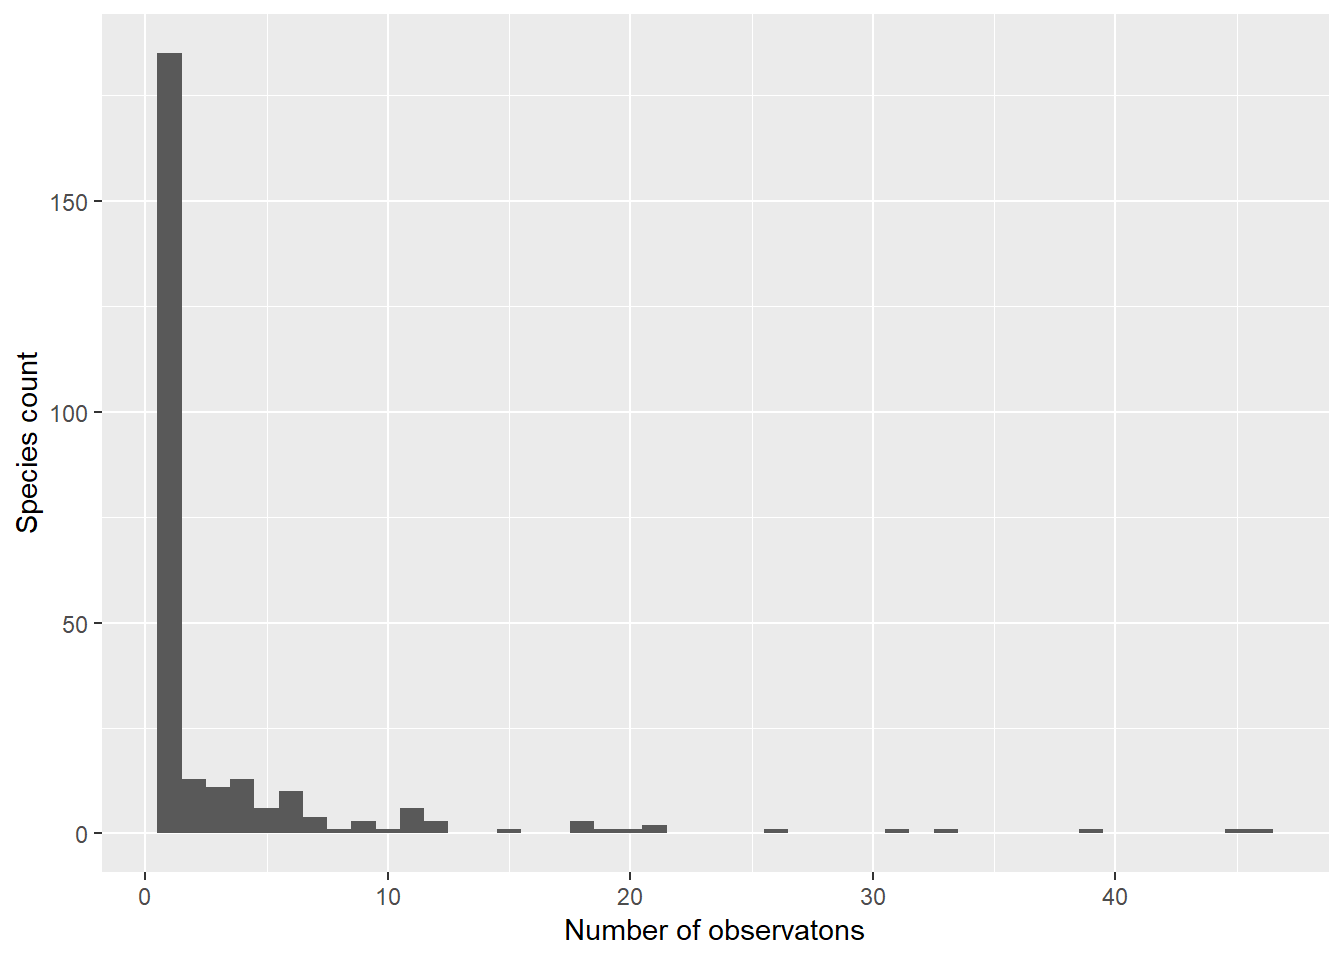
\includegraphics[width=0.5\textwidth]{master-thesis_files/figure-latex/phosphorus-1} \caption{Histogram of the number of observations per species for Pmass. Most species are singletons.}\label{fig:phosphorus}
\end{figure}

\subsection{Distribution of traits for the newly inferred
species}\label{distribution-of-traits-for-the-newly-inferred-species}

We obtained a new set of 599 species means for Nmass, Pmass, wsg and
LMA. What appears obvious here is that the range of estimated species
means is more narrow that the one of raw species means, estimated on the
dataset we performed the inference from. This is due to shrinkage of the
distributions by estimating hierarchically the species means
distribution, to keep only punctual estimators (the mean of the MCMC
sampled species means) as a final output. In more poetic terms, what
happens here is an illustration of the precaution principle: species
with extreme and with very few observations are attributed more
reasonable estimates, because of the uncertainties.
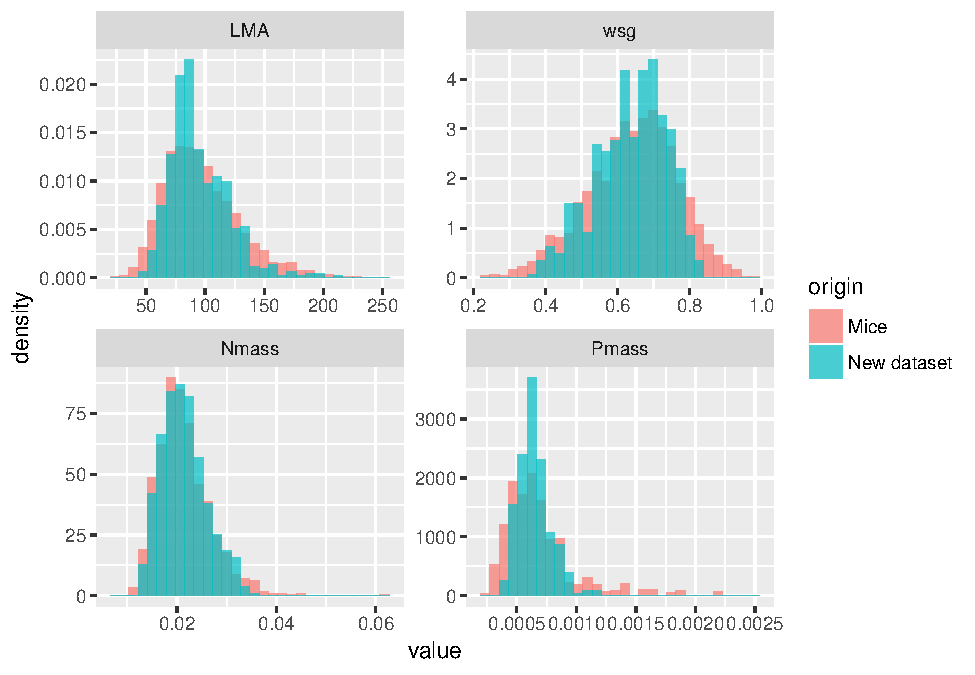
\includegraphics{master-thesis_files/figure-latex/unnamed-chunk-3-1.pdf}

\section{Appendix 3: Predictive mean matching (PMM)
explained}\label{appendix-3-predictive-mean-matching-pmm-explained}

Let \(X\) be a single variable that has cases with missing data, and a
set of variables \(Z\) (with no missing data) that are used to impute x.
PMM, as implemented on mice package, follows theses steps:

\begin{enumerate}
\def\labelenumi{\arabic{enumi}.}
\tightlist
\item
  For cases with no missing data, it estimates a linear regression of
  \(X\) on \(Z\), producing a set of coefficients \(\beta\).
\item
  It then makes a random draw from the ``posterior predictive
  distribution'' of \(\beta\), producing a new set of coefficients
  \(\beta*\). This would typically be a random draw from a multivariate
  normal distribution with mean \(\beta\), and the estimated covariance
  matrix of \(\beta\) (with an additional random draw for the residual
  variance). This step aims at producing variability in the imputed
  values, and is common to all efficient methods for multiple
  imputation.
\item
  Using \(\beta*\), it generates predicted values for \(x\) for all
  cases, both those with data missing on \(x\) and those with data
  present.
\item
  For each case with missing \(x\), if identifies a set of cases with
  observed \(X\) whose predicted values are close to the predicted value
  for the case with missing data.
\item
  It then randomly chooses one and assign its observed value to
  substitute for the missing value.
\item
  Steps 2 through 5 are then repeated for each completed data set.
\end{enumerate}

There are several variations to this method. Generally, each case with
missing data on \(X\) is matched to the \(k\) cases (with data present)
that have the closest predicted values, of which one is chosen at random
and its \(X\) value assigned to the case with missing data. We used the
default \(k=5\) proposed in the mice package and repeated the imputation
10 times, then pooled the datasets and averaged the obtained proposals
for missing values.

\section{Appendix 4: Complementary fuelwood
graphics}\label{appendix-4-complementary-fuelwood-graphics}

\begin{figure}
\centering
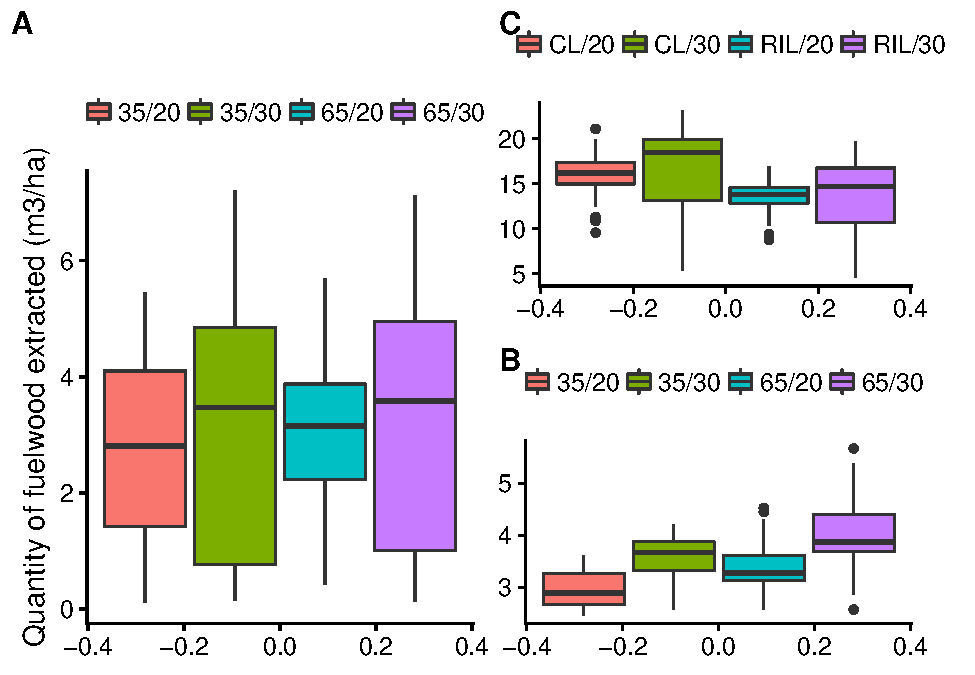
\includegraphics{master-thesis_files/figure-latex/fuelwood2-1.pdf}
\caption{\label{fig:fuelwood2}Estimated usable fuelwood volumes during the 2
firsts cutting cycles, originating from : A - Rotten trees, with a
comparison between cutting cycle durations (35 or 65), and target
volumes (20 or 30); B - Main tracks, with the same label correspondence
as A; and C - Secondary track, with separation on logging techniques (CL
or RIL) and target volumes (20 or 30); Black horizontal lines point the
median of the distributions. Color boxes encompass values between the
1st and 3rd quartile. Black points are extreme values.}
\end{figure}

The average usable fuelwood quantities (Figure \ref{fig:fuelwood2}) over
the two first cutting cycles, range mainly between 1 and 5 cubic meters
per hectare from rotten trees, and between 2 and 4 \(m^3/ha\) from main
track damages. Secondary tracks are the main potential source of
extractible fuelwood over two cutting cycles, with quantities ranging
from 10 to 20 \(m^3\) in most cases. The target volume is the principal
factor influencing this quantity for the main track, because its extent
depends on it. The duration of the cutting cycle has an impact, yet
marginal, due to longer regrowth period. Concerning secondary tracks, CL
obviously yields more damages than RIL, thus a higher quantity of
reusable wastes. No factor apparently influenced the fuelwood quantities
from rotten trees over two harvests, because of the quantity of
designated trees that vary between both cutting cycles, due to the lack
of stock regeneration exposed above. In fact, for the first rotation
only it depends directly on the target volume.

\begin{figure}
\centering
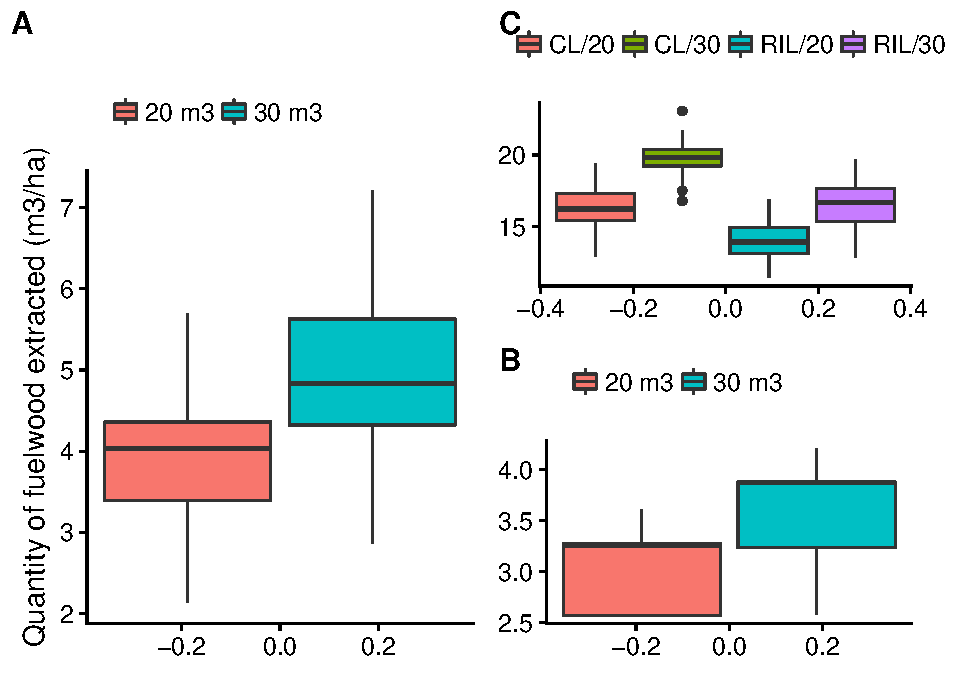
\includegraphics{master-thesis_files/figure-latex/fuelwoodsupp-1.pdf}
\caption{\label{fig:fuelwoodsupp}Same fuelwood estimates only for the first
curring cycle. A - Rotten trees, with a comparison between target
volumes (20 or 30); B - Main tracks, with the same label correspondence
as A; and C - Secondary track, with separation on logging techniques (CL
or RIL); Black horizontal lines point the median of the distributions.
Color boxes encompass values between the 1st and 3rd quartile. Black
points are extreme values.}
\end{figure}

\section{Appendix 5: Mortality curve for
Paracou}\label{appendix-5-mortality-curve-for-paracou}

\begin{figure}
\centering
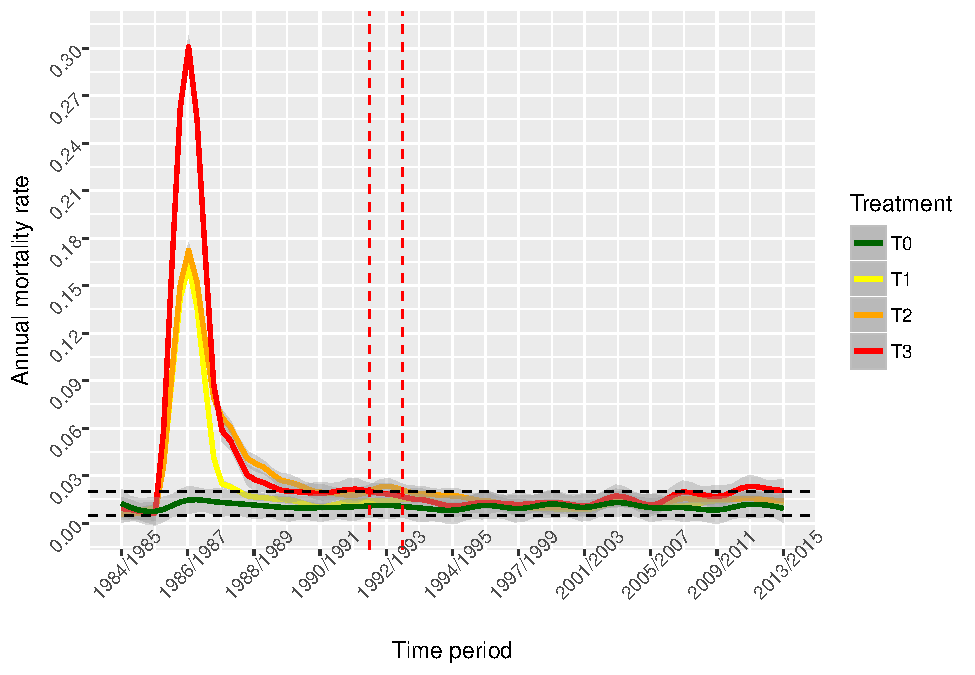
\includegraphics{master-thesis_files/figure-latex/mortality-1.pdf}
\caption{\label{fig:mortality}Annual mortality rates at Paracou plots,
pooled by treatment. T0 are control plots, T1 are conventionally logged
plots, T2 are logged plots with additional Stand Improvement treatment
(thinning by poison girdling), T3 are plots logged for timber and
additional fuelwood, having also undergone Stand Improvement treatments.
Grey bands around the curves are pseudo-confidence intervals generated
with geom\_smooth (package ggplot2). The plots were logged in
1986/1987.}
\end{figure}

\addcontentsline{toc}{section}{References}
\bibliography{C:/Users/nino.page/Desktop/bibs/thesis.bib}
\listoftables
\listoffigures

% Last pages
  %Last page
  \newpage
  \scriptsize{
  \paragraph{Résumé :}
  Les forêts tropicales abritent la moitié de la biodiversité terrestre mondiale, fournissent d'importants services écosystémiques à l'humanité, et sont un important réservoir de carbone. Ces forêts font face à de nombreuses menaces, dont la déforestation à des fins agricoles, et l'exploitation forestière séléctive. Cette dernière a affecté ou affectera la majorité des forêts tropicales, et a longtemps été une pratique incontrôlée. La Gestion Forestière Durable a été mise en avant pour tenter de résoudre ce problème, s'appuyant notamment sur les principes de l'Exploitation à Faible Impact et des incitations financières, comme le programme REDD+. Cependant, certains auteurs ont remis en question la durabilité réelle d'une telle exploitation. Evaluer l'impact des pratiques forestières est une tâche difficile, au vu des échelles de temps impliquées. En complément des efforts de suivi, la modélisation peut s'avérer utile pour fournir un aperçu des effets de l'exploitation forestière à plus long terme.   
  TROLL est un modèle spatialement explicite, individu-centré, qui simule un grand nombre d'espèces d'arbres. TROLL offre d'intéressantes perspectives en écologie théorique et appliquée. Nous avons exploré le potentiel de ce modèle pour simuler l'exploitation sélective, et explorer la durabilité de plusieurs scénarios.  Nous avons commencé par paramétrer 547 espèces à partir de la base de données BRIDGE, pour simuler d'importantes étendues de forêt, et avons ensuite essayé de réaliser une évaluation et calibration des trajectoires post-coupe simulées, en partaint de données réelles. La calibration fut impossible à cause d'une mortalité éxagérée dans les forêts d'entrées, pendant les premières années de simulation. Nos analyses suggèrent que TROLL a une structure spatiale différente de celle de vraies forêts, peut être à cause d'une sur-estimation de la compétition pour la lumière, le rendant inadapté à simuler à partir de vraies données pour le moment. Nous avons adapté la version existante du module simulant l'exploitation dans TROLL, pour implémenter plusieurs pratiques et paramètres sylvicoles. Nous avons réalisé un premier jeu de simulations sur deux forêts ayant des volumes de départ contrastés, durant 5 rotations. Nos résultats indiquent que l'exploitation sélective, telle qu'elle est pratiquée en Guyane Française, pourrait mener à un épuisement des volumes totaux d'espèces commerciales, ainsi qu'a une baisse du stock de carbone au fil des récoltes, et cela même pour des rotations de 65 ans, avec des intensités de 20$m^3$ et les techniques de l'EFI. Ces résultats sont cependant préliminaires et manquent de réplication, ils doivent donc être interprétés avec précaution. Des analyses plus poussées sur des scénarios plus nombreux sont requises afin de confirmer et affiner nos résultats. TROLL, combiné avec le modèle d'exploitation que nous avons mis à jour, présente un potentiel promettent pour explorer différents scénarios sylvicoles, et répondre à des problématiques appliquées.
  \paragraph{Mots clés :} Gestion Forestière Durable, Simulation, Exploitation forestière, Modélisation, Modèle individu-centré.
  \paragraph{Abstract:}
  Tropical forests shelter half the terrestrial biodiversity worldwide, provide important services to humanity and are a major reservoir of carbon. These forests face numerous threats, among others deforestation for agriculture and selective logging. Selective logging affected or will affect the majority of tropical forest outside protected areas, and has long been an uncontroled predatory practice. Sustainable Forest Management (SFM) has been promoted to answer this issue, relying on Reduced Impact Logging, and financial incentives such ad REDD+. However, some authors asked whether these techniques are sustainable. Assessing the sustainability of Forest Management difficult task, because of the efforts needed by field studies, and time scales involved. To complement monitoring efforts, the use of models can provide valuable insights of longer-term effects of selective logging. TROLL is an individual-tree-based, spatially explicit forest model that uses functional traits to simulate the life cycle of a wide range of tree species. TROLL offers promising perspectives in studying ecological theories and applied problems. We explored the potential of this model to simulate selective logging and assess the sustainability of different scenarios. We preliminarily parametrized 547 species from the BRIDGE dataset to simulate large forest plots, and we attempted to evaluate and calibrate the simulated post-logging trajectories inputting real forest censuses in the model. The calibration was impossible because of exagerated mortality in the inputted forests during the first years of simulation. Spatial structure analysis suggest that TROLL has a different spatial structure than real forests, maybe due to overestimation of competition for light, thus making unadapted the use of real data inputs for now. We adapted the existing version of the module that simulates selective logging in TROLL, to implement cutting cycles, conventional logging, and designation based on timber interest ranks. We did a preliminary set of simulations on two forests that had contrasted timber volumes, to assess the importance of silviculture parameters over five cutting cycles. Our results indicate that selective logging, as applied in French Guiana and neighboring countries, may lead to a depletion of total timber stocks and high-grade species, along with a decrease of carbon stocks over harvests, even for 65 years cutting cycles with 20$m^3$ harvested and RIL techniques. However, our results are preliminary, lack replication, and thus have to be interpreted carefully. Further, extensive analyses are needed to confirm and refine our findings. TROLL, combined with the logging model we updated, has a promising potential to explore a wide range of silviculture scenarios, and adress applied problematics.
  \paragraph{Keywords:}Sustainable Forest Management, Simulation, Selective logging, Modeling, Individual-based model.
  }
  
  \vspace*{\fill}
  
\includegraphics{images/logo}

\end{document}
